\documentclass[twoside,openright,a4paper,11pt,french]{article}
\usepackage[utf8]{inputenc}
\usepackage[french]{babel}
\usepackage[T1]{fontenc}
\usepackage{emptypage}
\usepackage{amsmath}
\usepackage{amssymb}

% Utilisation d'url
\usepackage{url}
\urlstyle{sf}

% Utilisation d'images, stockées dans le répertoire ./pics/
\usepackage{graphicx}
\graphicspath{pics/}

% Définition des marges
\usepackage{geometry}
\geometry{
  left=25mm,
  right=25mm,
  top=25mm,
  bottom=25mm,
  foot=15mm
}
\usepackage{listings}
\usepackage{color}

\definecolor{gray}{rgb}{0.8,0.8,0.8}

\begin{document}

\pagestyle{plain}
\setlength{\parindent}{0pt}
% La page de garde
\thispagestyle{empty}

\begin{center}
       \noindent
       
\includegraphics[height=2.5cm]{./pics/uds.eps}       
       
       \vfill\vfill

    {\large \textsc{Licence 3 de Sciences, mention Informatique}}

    \bigskip\bigskip

    {\large \textsc{Intelligence Artificielle}}

    \vfill\vfill

% Titre du document
    {\huge \sc
      \begin{center} 
        Rapport sur le projet: \\
        Perceptron et perceptron multi-couchers avec Neuroph
      \end{center}}

    \vfill\vfill

    {\large Présenté par}

\medskip

% Identité des auteurs
    {\large Victor \textsc{Constans}}\\
    {\large Luigi  \textsc{Coniglio}}\\
\bigskip

\end{center}



% La table des matières
\parskip=0pt
\tableofcontents
\clearpage


\vspace{5cm}

%Start content

\section{Fonctions booléennes}

Dans la première section de ce rapport on se propose
d'implementer des fonctions booléennes a l'aide des réseaux
de neurones. 

\subsection{"Et" logique}

En matematique la conjonction logique $\land$ est un
connecteur logique que, étant donné deux propositions $a$ et $b$
forme une nouvelle propositions $a \land b$ qui est vrai seulement
si $a$ et $b$ sont vraies.

\begin{table}[h]
  \centering
  \begin{tabular}{| c | c | c |}
    \hline
    \textbf{$a$} & \textbf{$b$} & \textbf{$a \land b$}\\
    \hline
    0 & 0  & 0 \\
    \hline
    0 & 1  & 0 \\
    \hline
    1 & 0  & 0 \\
    \hline
    1 & 1  & 1 \\
    \hline
  \end{tabular}
  \caption{Table de vérité de $a \land b$}
  \label{tab:et}
\end{table}




\subsubsection{Un perceptron pour $\land$} 

Est il possible d'utiliser un perceptron pour apprendre la fonction logique
"et"? Bien sur, en effet même un perceptron mono-couche est suffisant pour
obtenir ce resultat.\\

Le perceptron peut être utilisé comme un classificateur linéaire, c'est-à-dire l'algorithme du
perceptron permettant de reconnaitre et donc classifier des données (ou points)
linéairement séparables.\\

Un ensemble de points dans le plan caractérisé par deux sous-classes disjointes
de points, est dit linéairement séparable si il éxiste une droite qui sépare
complétement les deux sous-classes.\\

En trois dimension, un ensemble est linéairement séparable si il éxiste un plan
qui sépare les deux classes. En quatre ou plus dimensions on ne parlera plus de
plan mais d'hyperplan.


\begin{figure}[h]
\centering
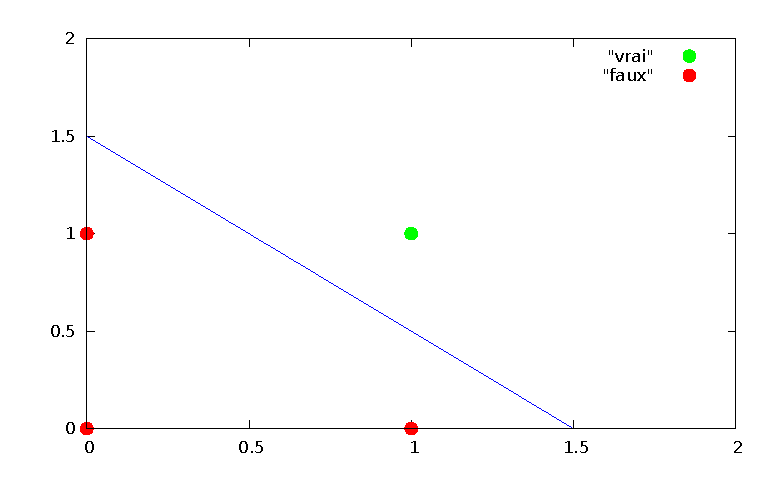
\includegraphics[width=10cm]{./pics/and/and.eps}
\caption{La fonction logique "et" est linéairement séparable}
\label{fig:and}
\end{figure}


Comme montre la figure \ref{fig:and} la fonction "et" est bien linéairement
séparable. Etant donné que tout ensemble linéairement séparable peut être
discriminé par un perceptron monocouche, on est sûr de pouvoir trouver un perceptron monocouche qui
engendre la fonction booléenne $\land$.\\

Le perceptron créé avec Neuroph qu'on utilisera pour cette fonction 
est très simple et est illustré dans la figure \ref{fig:per_and}.
Le data set pour l'apprentissage contiens les mêmes valeurs que la table
\ref{tab:et}.

\begin{figure}[h]
\centering
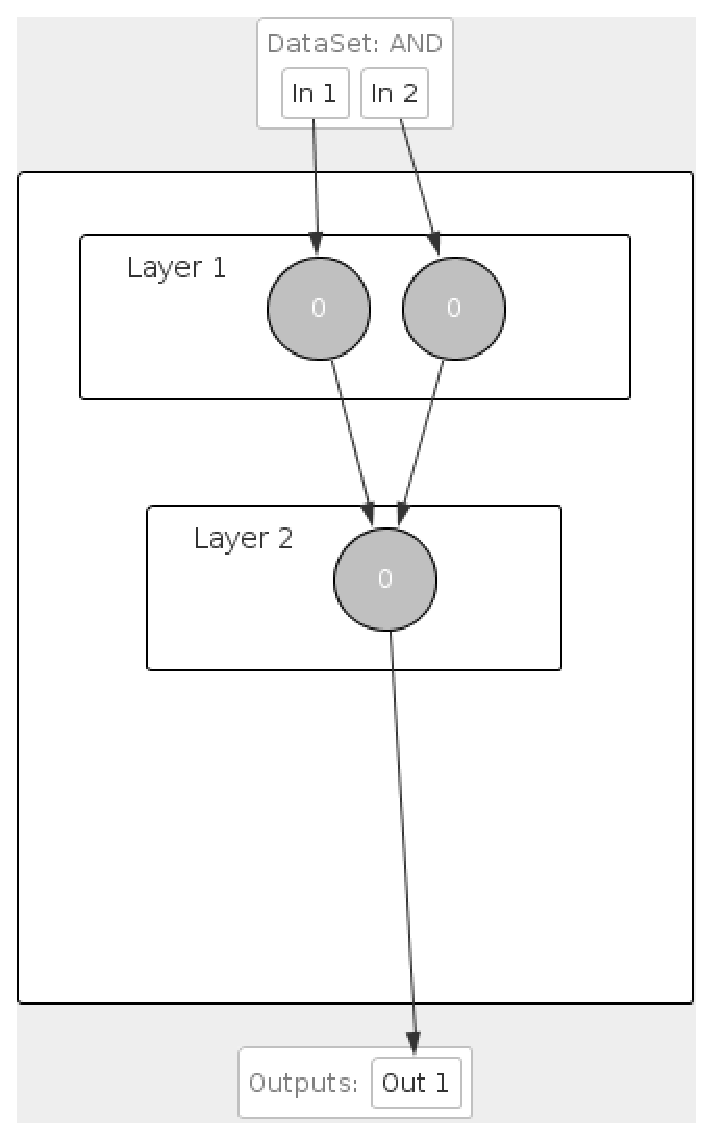
\includegraphics[width=4.5cm,height=7cm]{./pics/perc_and.eps}
\caption{Perceptron pour la fonction "et"}
\label{fig:per_and}
\end{figure}

Pendant l'entrainement du perceptron (dont les poids ont été initialisés
aléatoirement) avec un taux d'apprentissage de 0.2 (valeur par
défaut) on obtient une courbe d'apprentissage qui converge toujours à
zero. La forme de celle-ci dépendra essentiellement des valeurs initiales des
poids. 


\begin{figure}[h]
\centering
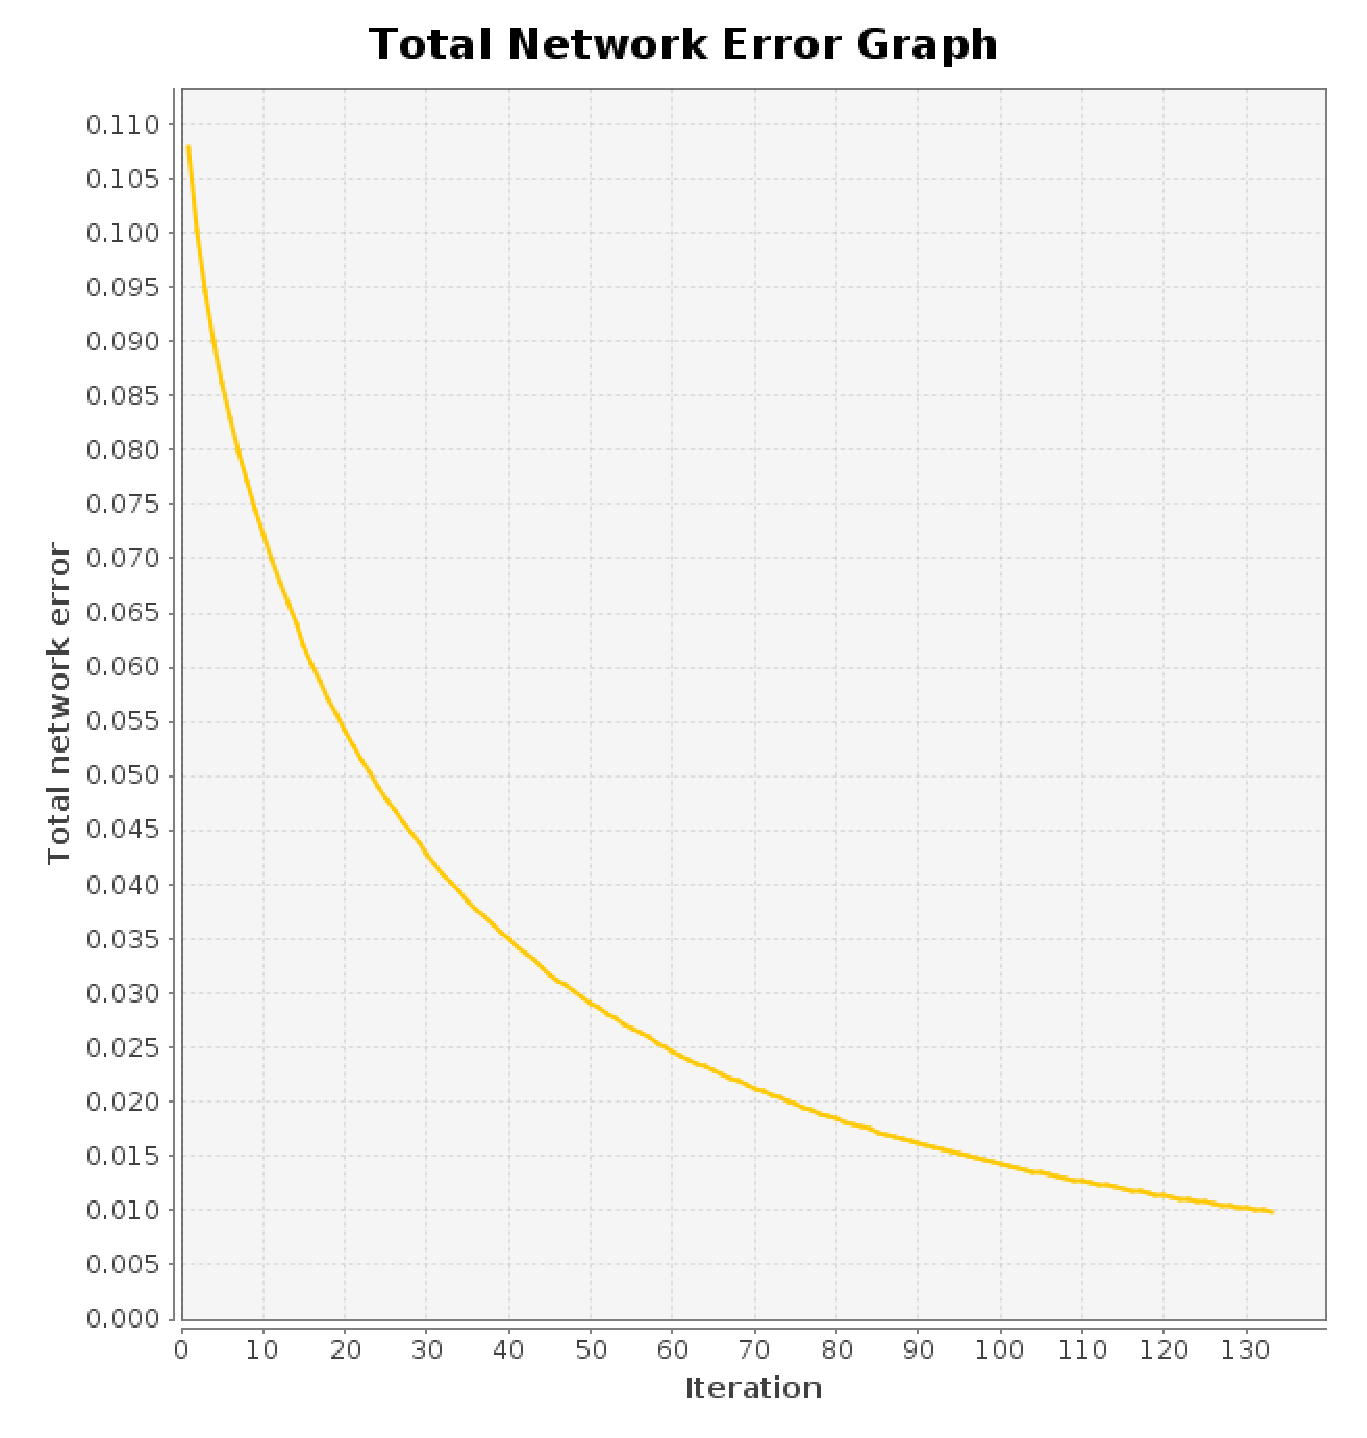
\includegraphics[width=12cm,height=9cm]{./pics/and_error1.eps}
\caption{Exemple de courbe d'apprentissage pour la fonction "et"}
\label{fig:anderr}
\end{figure}

La figure \ref{fig:anderr} montre un exemple de courbe d'apprentissage
obtenu avec les valeurs susmentionnées.\\

L'apprentissage peut être pensé comme le processus pendant lequel le
réseau de neurons cherche de s'approcher le plus possible du plus petit
taux d'erreur.\\

En effet, la meilleure configuration (valeurs des poids, biais, etc.) pour
notre réseau de neurones correspond au point de minimum globale de la fonction
$E$ qui associe à chaque configuration de notre réseau de neurones un coût $C$.\\

$E$ mesure la différence entre le valeur attendu et celle produite et est
souvent calculé comme étant $E(y,y') = \tfrac{1}{2} \lVert y-y'\rVert^2$ ou $y$ est
le valeur attendu et $y'$ est la valeur produite par le réseau.
Mais pourquoi $\lVert y-y'\rVert$ ne suffit simplement pas? 
En effet, la choix d'utiliser une fonction quadratique n'est pas un hasard. 
Un des problèmes les plus importants dans l'apprentissage supervivée d'un réseau
de neurones qui se base sur l'algorithme du gradient (gradient descent) est
celui posé par les points de minimum locales de $E$. Le fait que $E$ soit
quadratique permet d'exploiter la convexité des fonctions quadratique pour
minimiser ce probleme. Le $\tfrac{1}{2}$ permet de simplifier la fonction lors
de sa dérivation.\\

Comme attendu, dans notre cas le perceptron n'a aucun problème à trouver le
minimum globale de $E$, mais dans ce premiere exemple on se contente d'entrainer le
réseau de neurones jusqu'à obtenir un taux d'erreur moyen de seulement 1\%. La
figure \ref{fig:andtest1} montre les résultats de l'entrainement:

\begin{figure}[h]
\centering
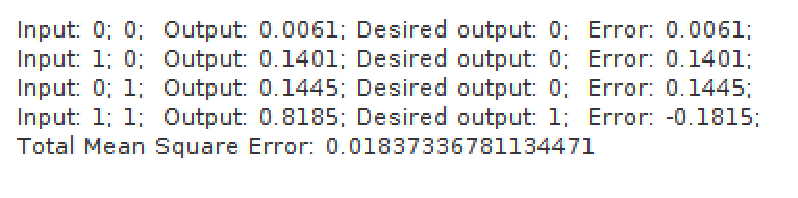
\includegraphics[width=7.3cm,height=2.3cm]{./pics/andtest1.eps}
\caption{Test du perceptron après l'apprentissage de la fonction "et"}
\label{fig:andtest1}
\end{figure}

En utilisant la definition de $E$ on peut vérifier que le coût
moyen est bien proche de $0.01$:

\begin{equation*}
  \begin{aligned}
  \tfrac{1}{4}\times(E(0,0.0061)+E(0,0.1401)+E(0,0.1445)+E(1,0.8185))\\
  = \tfrac{1}{4}\times(\tfrac{0.0061^2}{2}+\tfrac{0.1401^2}{2}+\tfrac{0.1445^2}{2}+\tfrac{0.1815^2}{2}) =
  0.009185965
  \end{aligned}
\end{equation*}

Le resultat obtenu est très proche de celui souhaité, en effet il suffit 
d'introduire un seuil pour obtenir un output qui soit à 0 ou à 1.
Dans Neuroph cela se traduit par l'utilisation de la fonction d'activation step pour le
neurone d'output.


\begin{figure}[h]
\centering
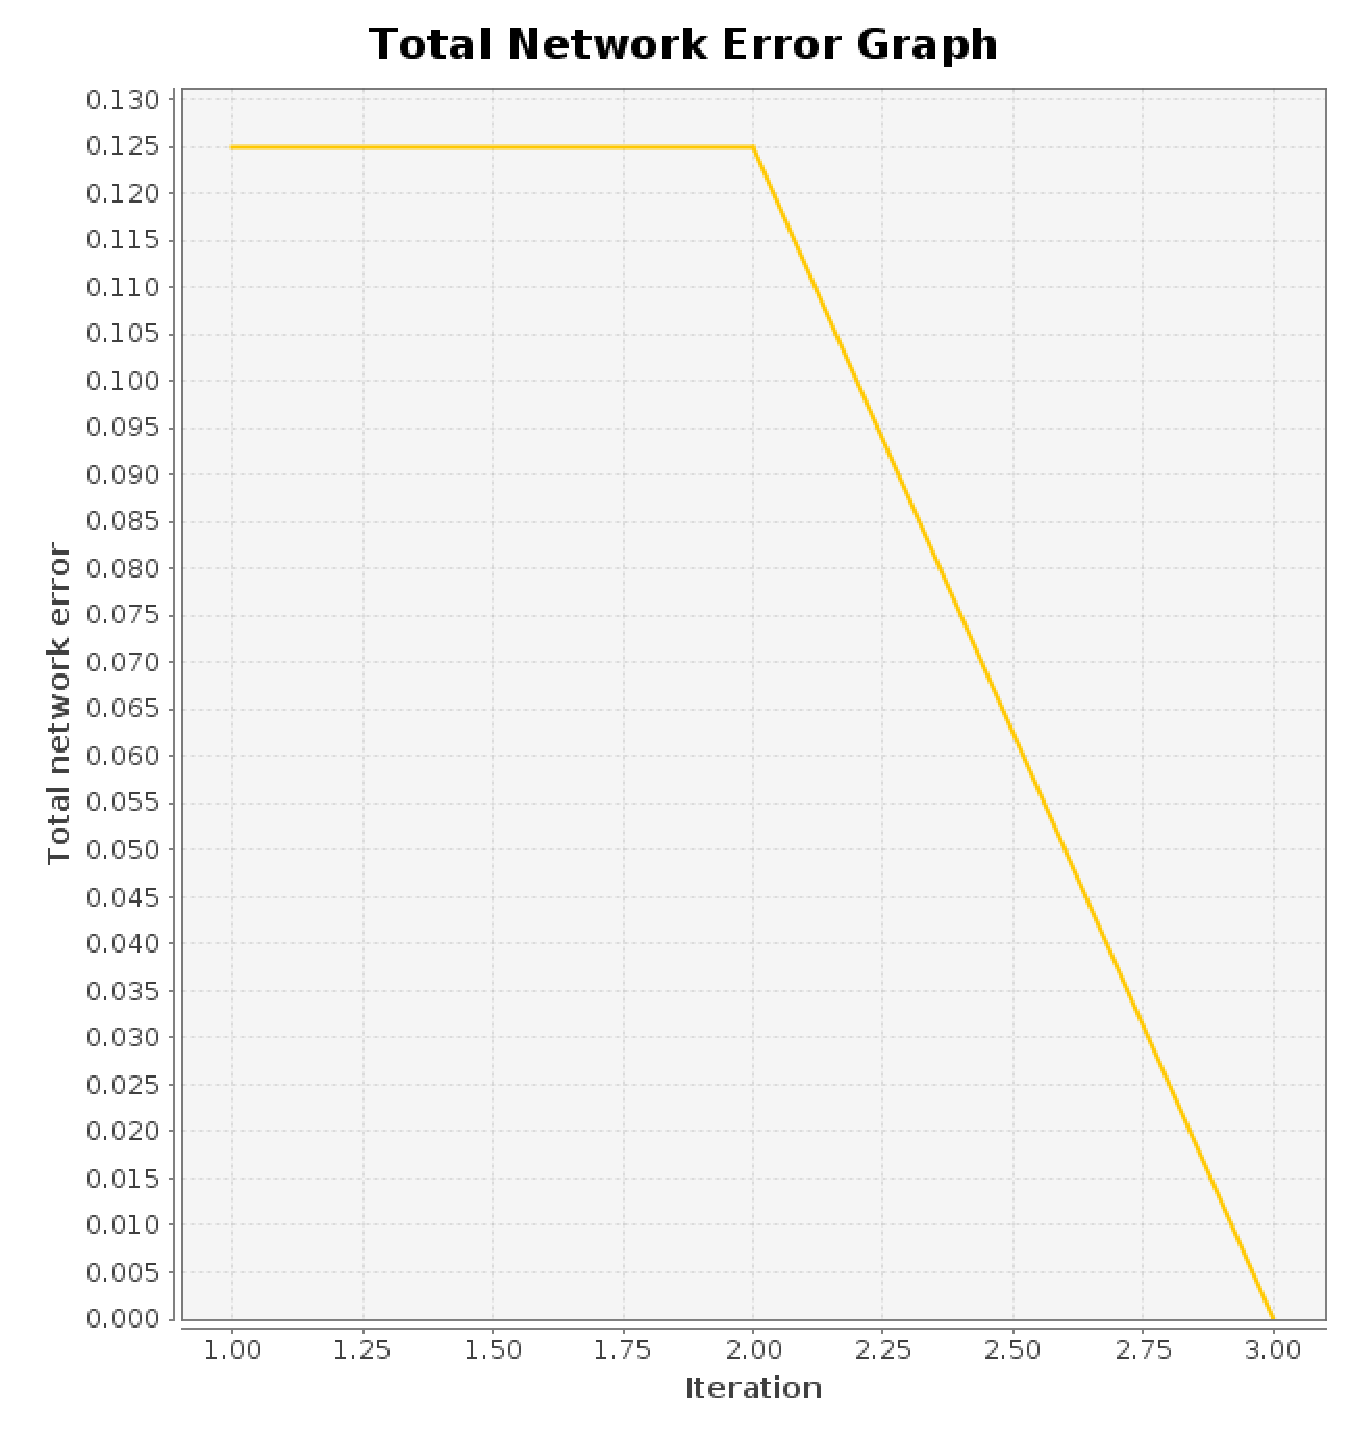
\includegraphics[width=12cm,height=9cm]{./pics/and_error2.eps}
\caption{Courbe d'apprentissage de "et" en utilisant la fonction step}
\label{fig:anderr}
\end{figure}



Cette technique nous permet d'obtenir une sortie parfaite qui ne présente
aucun taux d'erreur.



\begin{figure}[h]
\centering
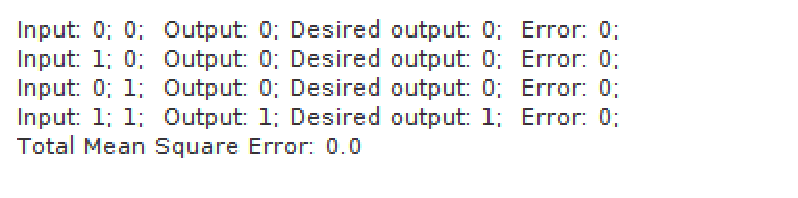
\includegraphics[width=7.3cm,height=2.3cm]{./pics/andtest2.eps}
\caption{Test d'erreur après l'apprentissage de la fonction "et"}
\label{fig:andtest2}
\end{figure}


\subsubsection{Differents pas d'apprentissage}

Le pas d'apprentissage détermine la vitesse (pas) avec laquelle notre réseau
cherche à s'approcher du point d'erreur minimum. 
A chaque époque ({\it batch learning}) ou itération ({\it incremental
learning}) les poids du réseau sont mise à jour en utilisant une combinaison du
pas d'apprentissage et du gradient $\nabla E$ ce qui indique la direction du taux
d'accroissement le plus élevé de $E$ et sa pente.\\

Le pas d'apprentissage joue un rôle très important dans la recherche du
minimum globale d'une fonction. 
Si un pas d'apprentissage est trop grand, cela risque de ne pas atteindre le minimum globale.
Inversement, un pas trop petit augmente le temps nécessaire pour entrainer le réseau et risque de
se bloquer dans un point de minimum locale.\\

Dans notre cas le changement du pas d'apprentissage n'a aucun effet que celui 
de changer la vitesse d'apprentissage.


\begin{figure}[h]
\centering
\includegraphics[width=12cm,height=9cm]{./pics/and_error3.eps}
\caption{Apprentissage fonction "et" avec un pas de 0.1}
\label{fig:anderr3}
\end{figure}

\begin{figure}[h]
\centering
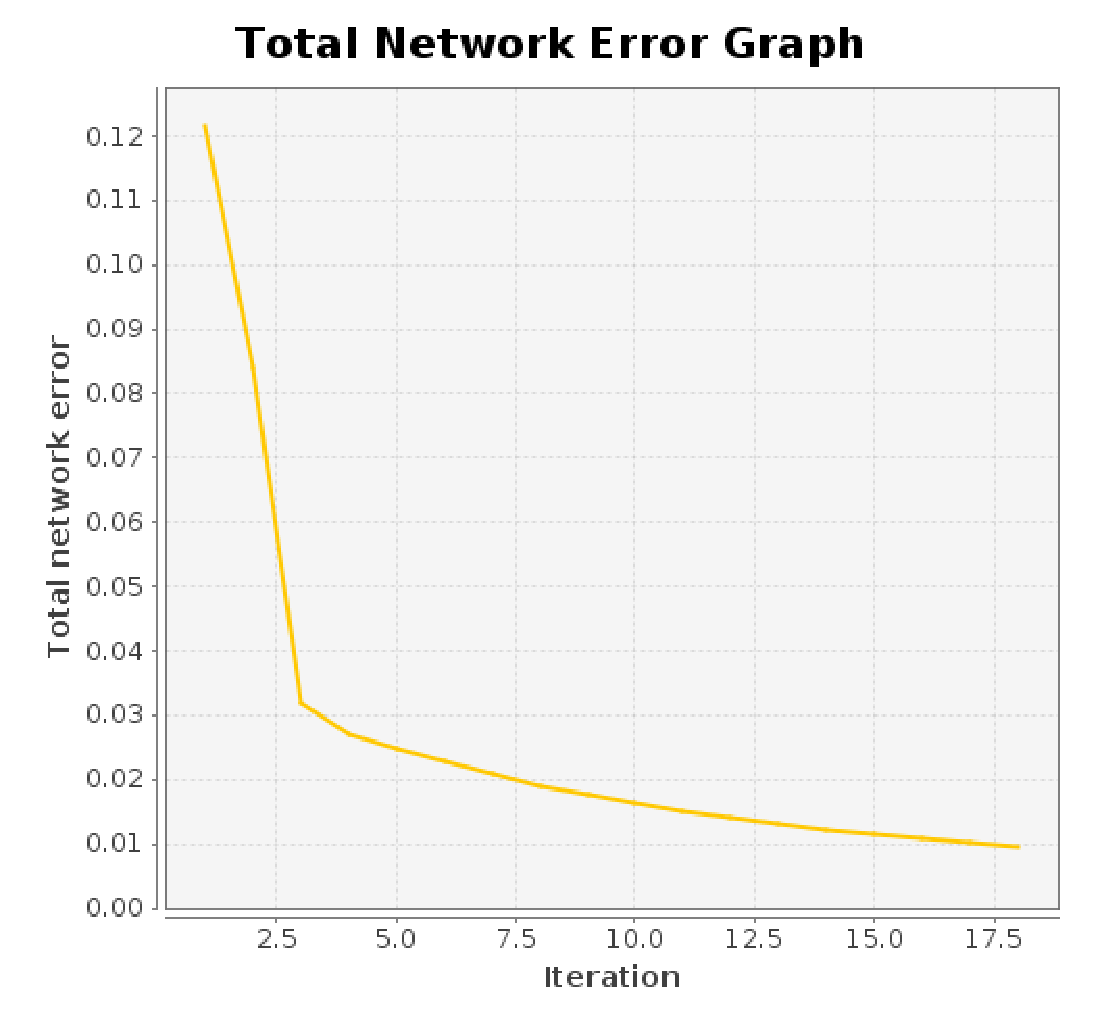
\includegraphics[width=12cm,height=9cm]{./pics/and_error4.eps}
\caption{Apprentissage fonction "et" avec un pas de 1}
\label{fig:anderr4}
\end{figure}

Avec un pas de 1 (figure \ref{fig:anderr4}) l'erreur totale du perceptron
tombe en-dessous de 0.01 après seulement 17 itérations. En revanche avec 
un pas de 0.1 le nombre d'itérations nécessaires pour obtenir le même
résultat monte à plus de 155 itérations (figure \ref{fig:anderr3}).

\subsection{Equivalence logique}
En matematique deux propositions sont dites equivalentes si l'un implique
l'autre: $a \Leftrightarrow b$. La table de verite de l'equivalence logique
est illustre par la table \ref{tab:eq}.
Cette table de vérité nous servira de data set pour l'entrainement de tout
les perceptron de cette partie.


\begin{table}[h]
  \centering
  \begin{tabular}{| c | c | c |}
    \hline
    \textbf{$a$} & \textbf{$b$} & \textbf{$a \Leftrightarrow b$}\\
    \hline
    0 & 0  & 1 \\
    \hline
    0 & 1  & 0 \\
    \hline
    1 & 0  & 0 \\
    \hline
    1 & 1  & 1 \\
    \hline
  \end{tabular}
  \caption{Table de verite de $a \Leftrightarrow b$}
  \label{tab:eq}
\end{table}

\subsubsection{Un perceptron monocouche pour $\Leftrightarrow$}

Comme pour la fonction booléenne "et" précédente nous allons essayer de faire apprendre
l'équivalence à un perceptron monocouche. Nous avons donc créé un perceptron monocouche
avec deux inputs et un output

\begin{figure}[h]
\centering
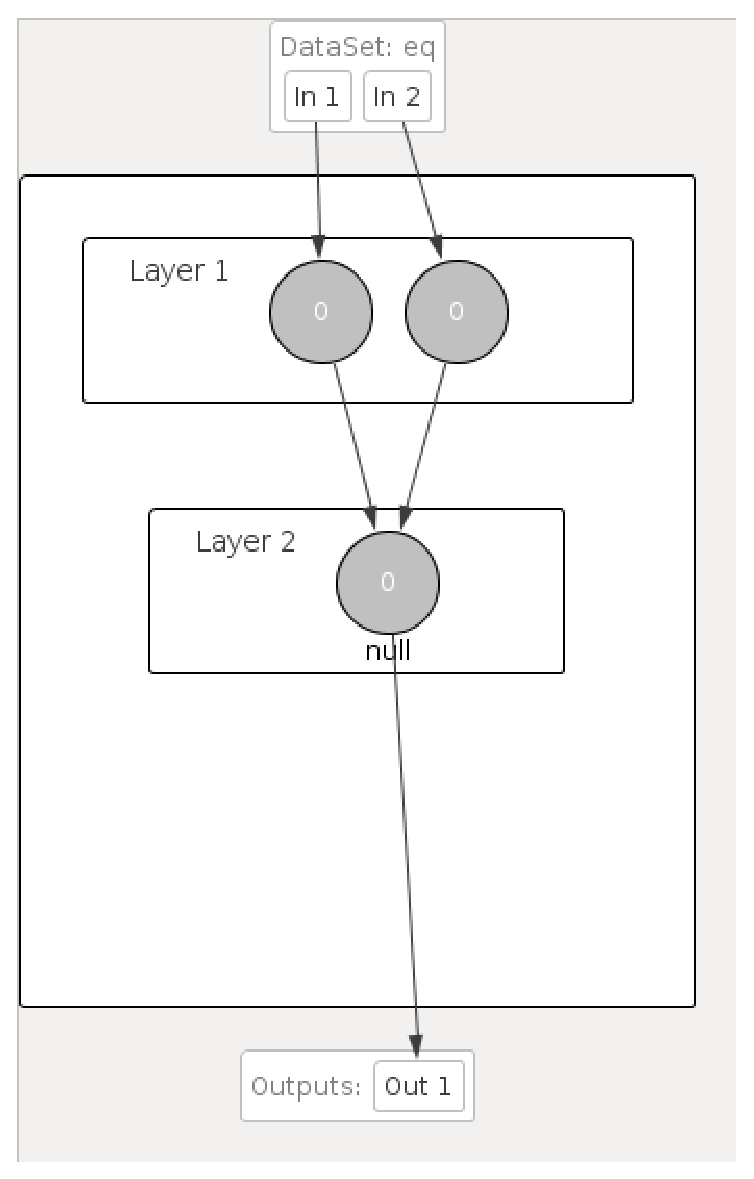
\includegraphics[width=5cm,height=7cm]{./pics/eq/perceptron_mono.eps}
\caption{Apprentissage fonction "et" avec un pas de 1}
\label{fig:anderr4}
\end{figure}

Entrainons ce perceptron avec le data set sur 1000 itérations.

\begin{figure}[h]
\centering
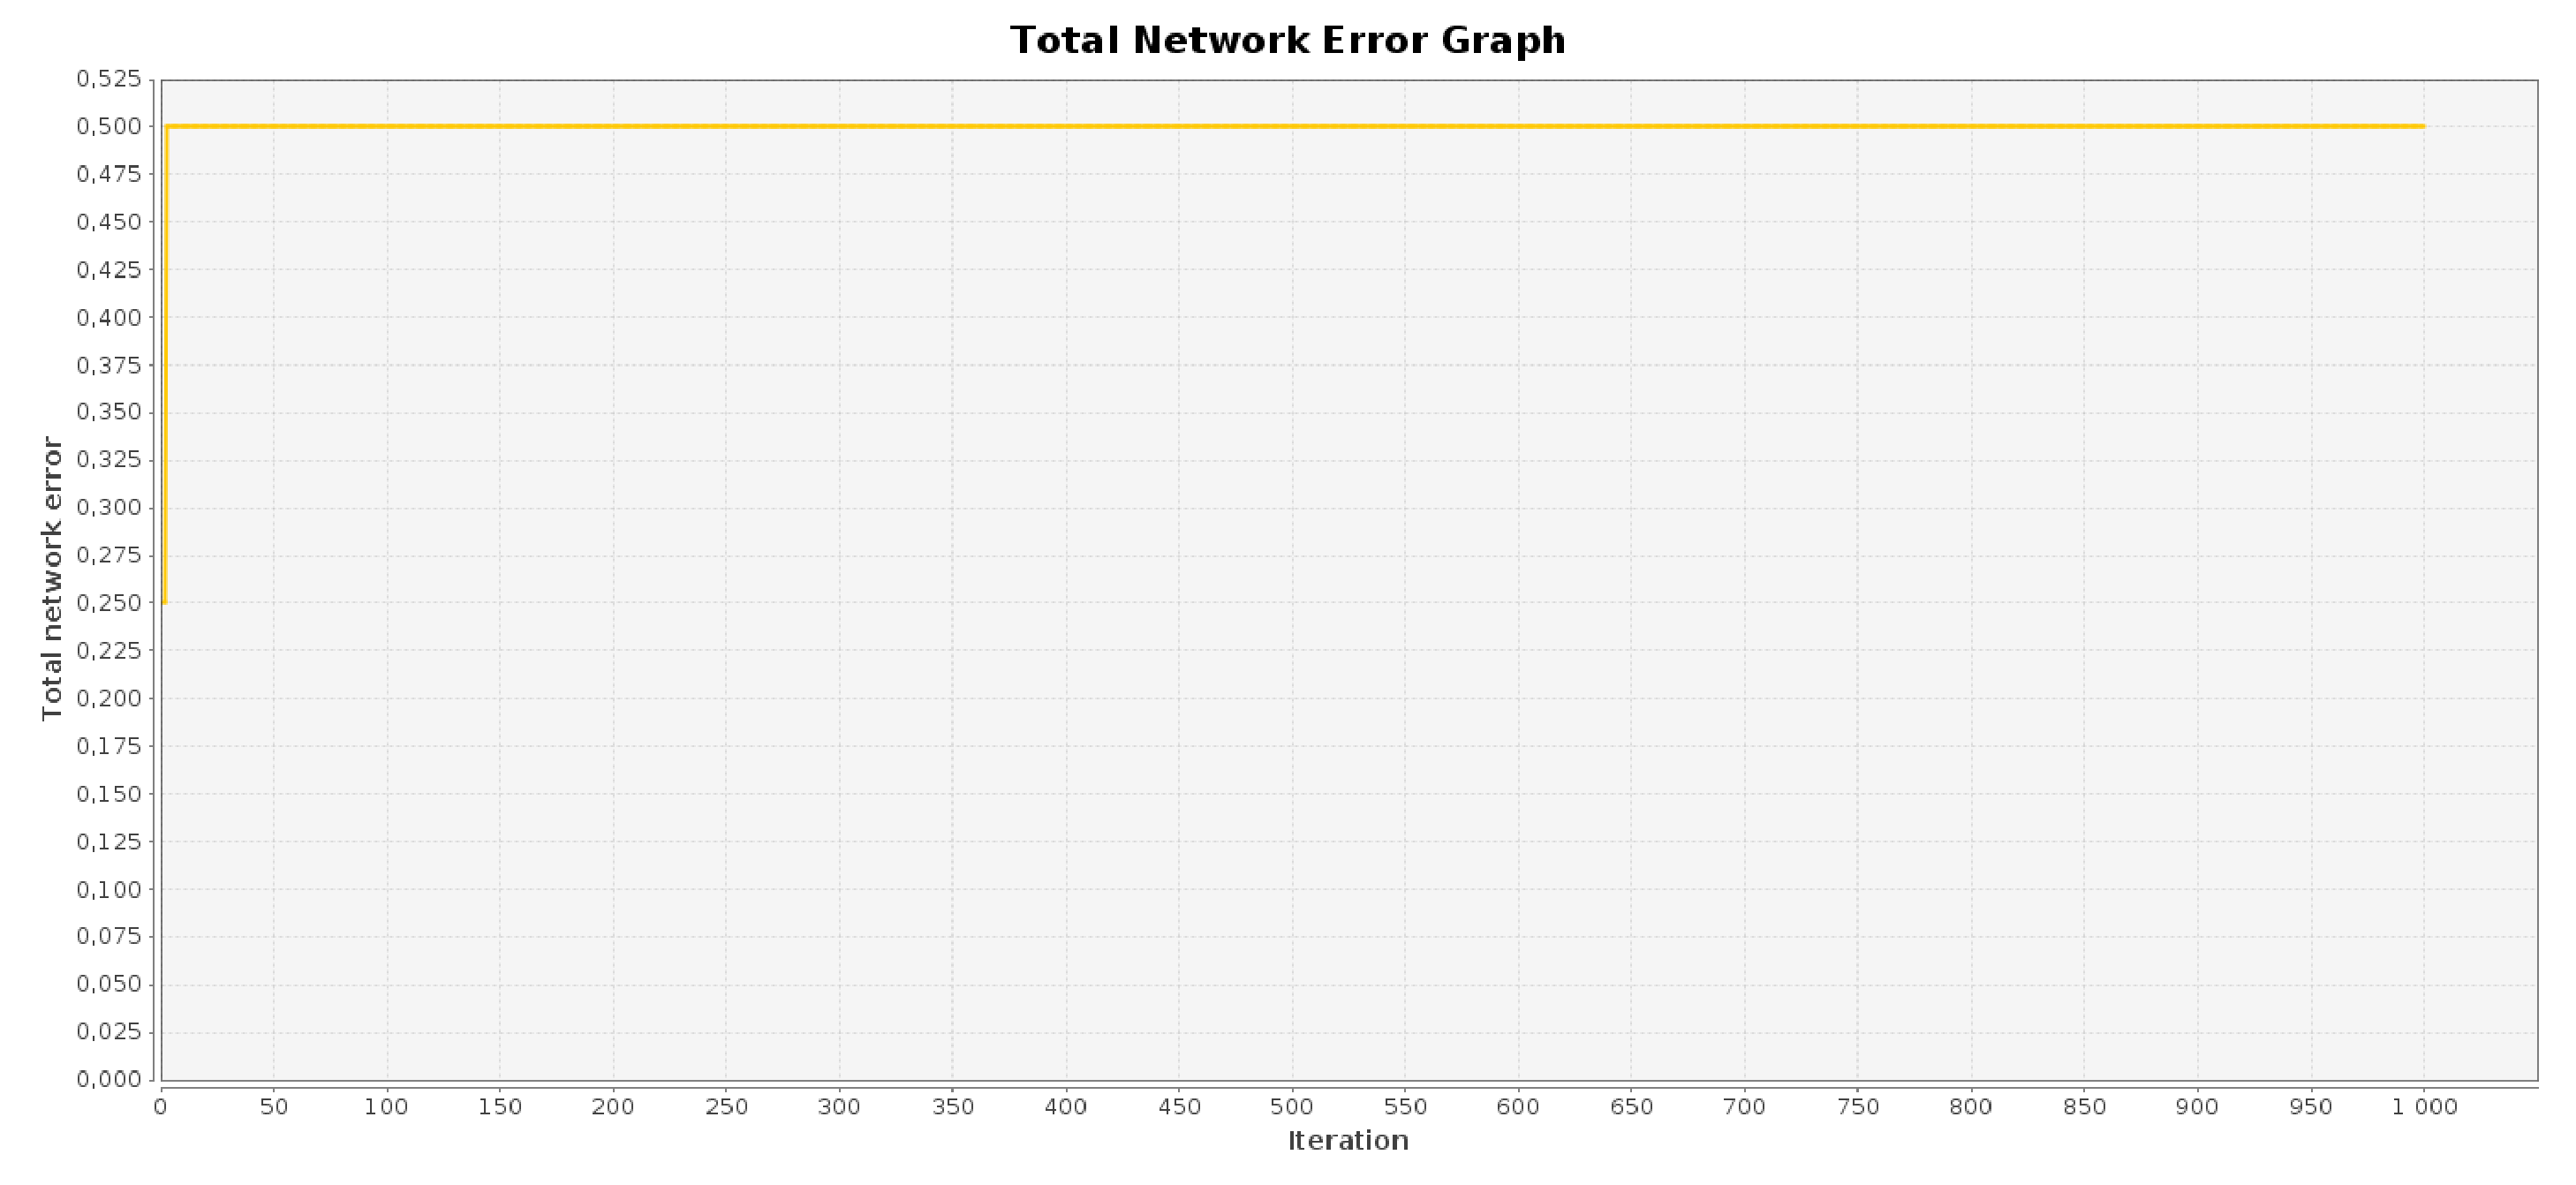
\includegraphics[width=12cm,height=9cm]{./pics/eq/mono_eq_def.eps}
\caption{Apprentissage fonction "et" avec un pas de 1}
\label{fig:anderr4}
\end{figure}

Nous pouvons observer qu'il ne semble pas avoir de convergence avec ce perceptron
en laissant les paramètre par défaut.
Nous pouvons changer le pas d'apprentissage pour essayer d'avoir
une convergence.

Voyons se que cela donne avec des pas d'apprentissage de respectivement 0.1 , 0.01 , 0.001.

\begin{figure}[h]
\caption{Apprentissage fonction "et" avec un pas de 1}
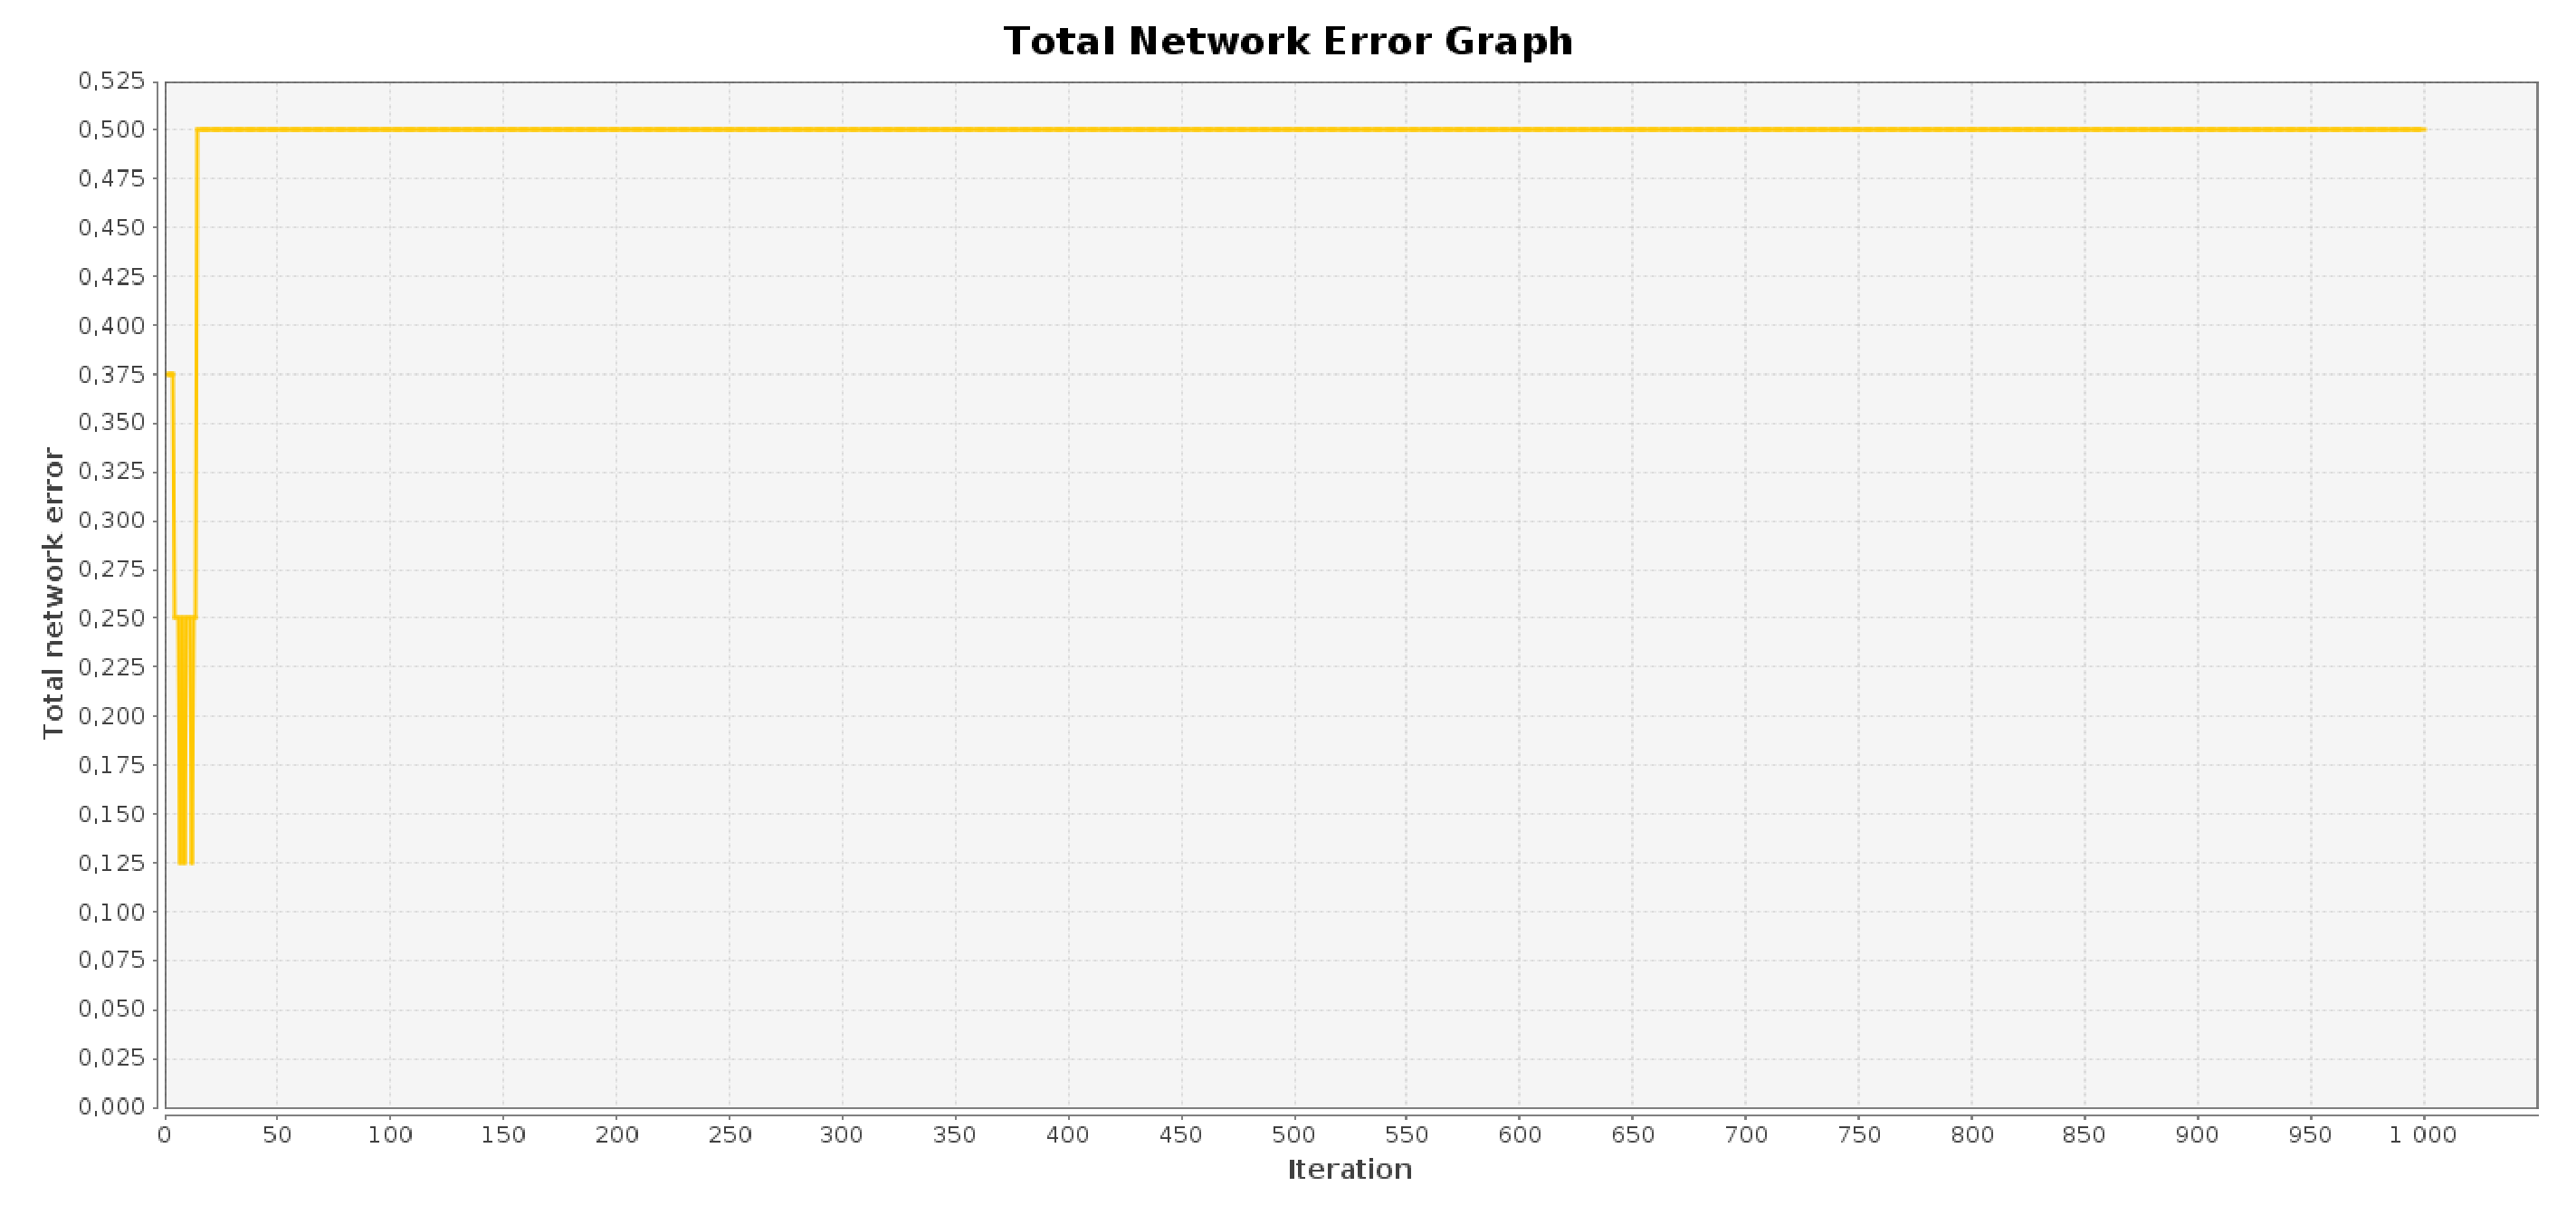
\includegraphics[width=6cm,height=3cm]{./pics/eq/mono_eq_0.1.eps}
\label{fig:anderr4}
\end{figure}

\begin{figure}[h]
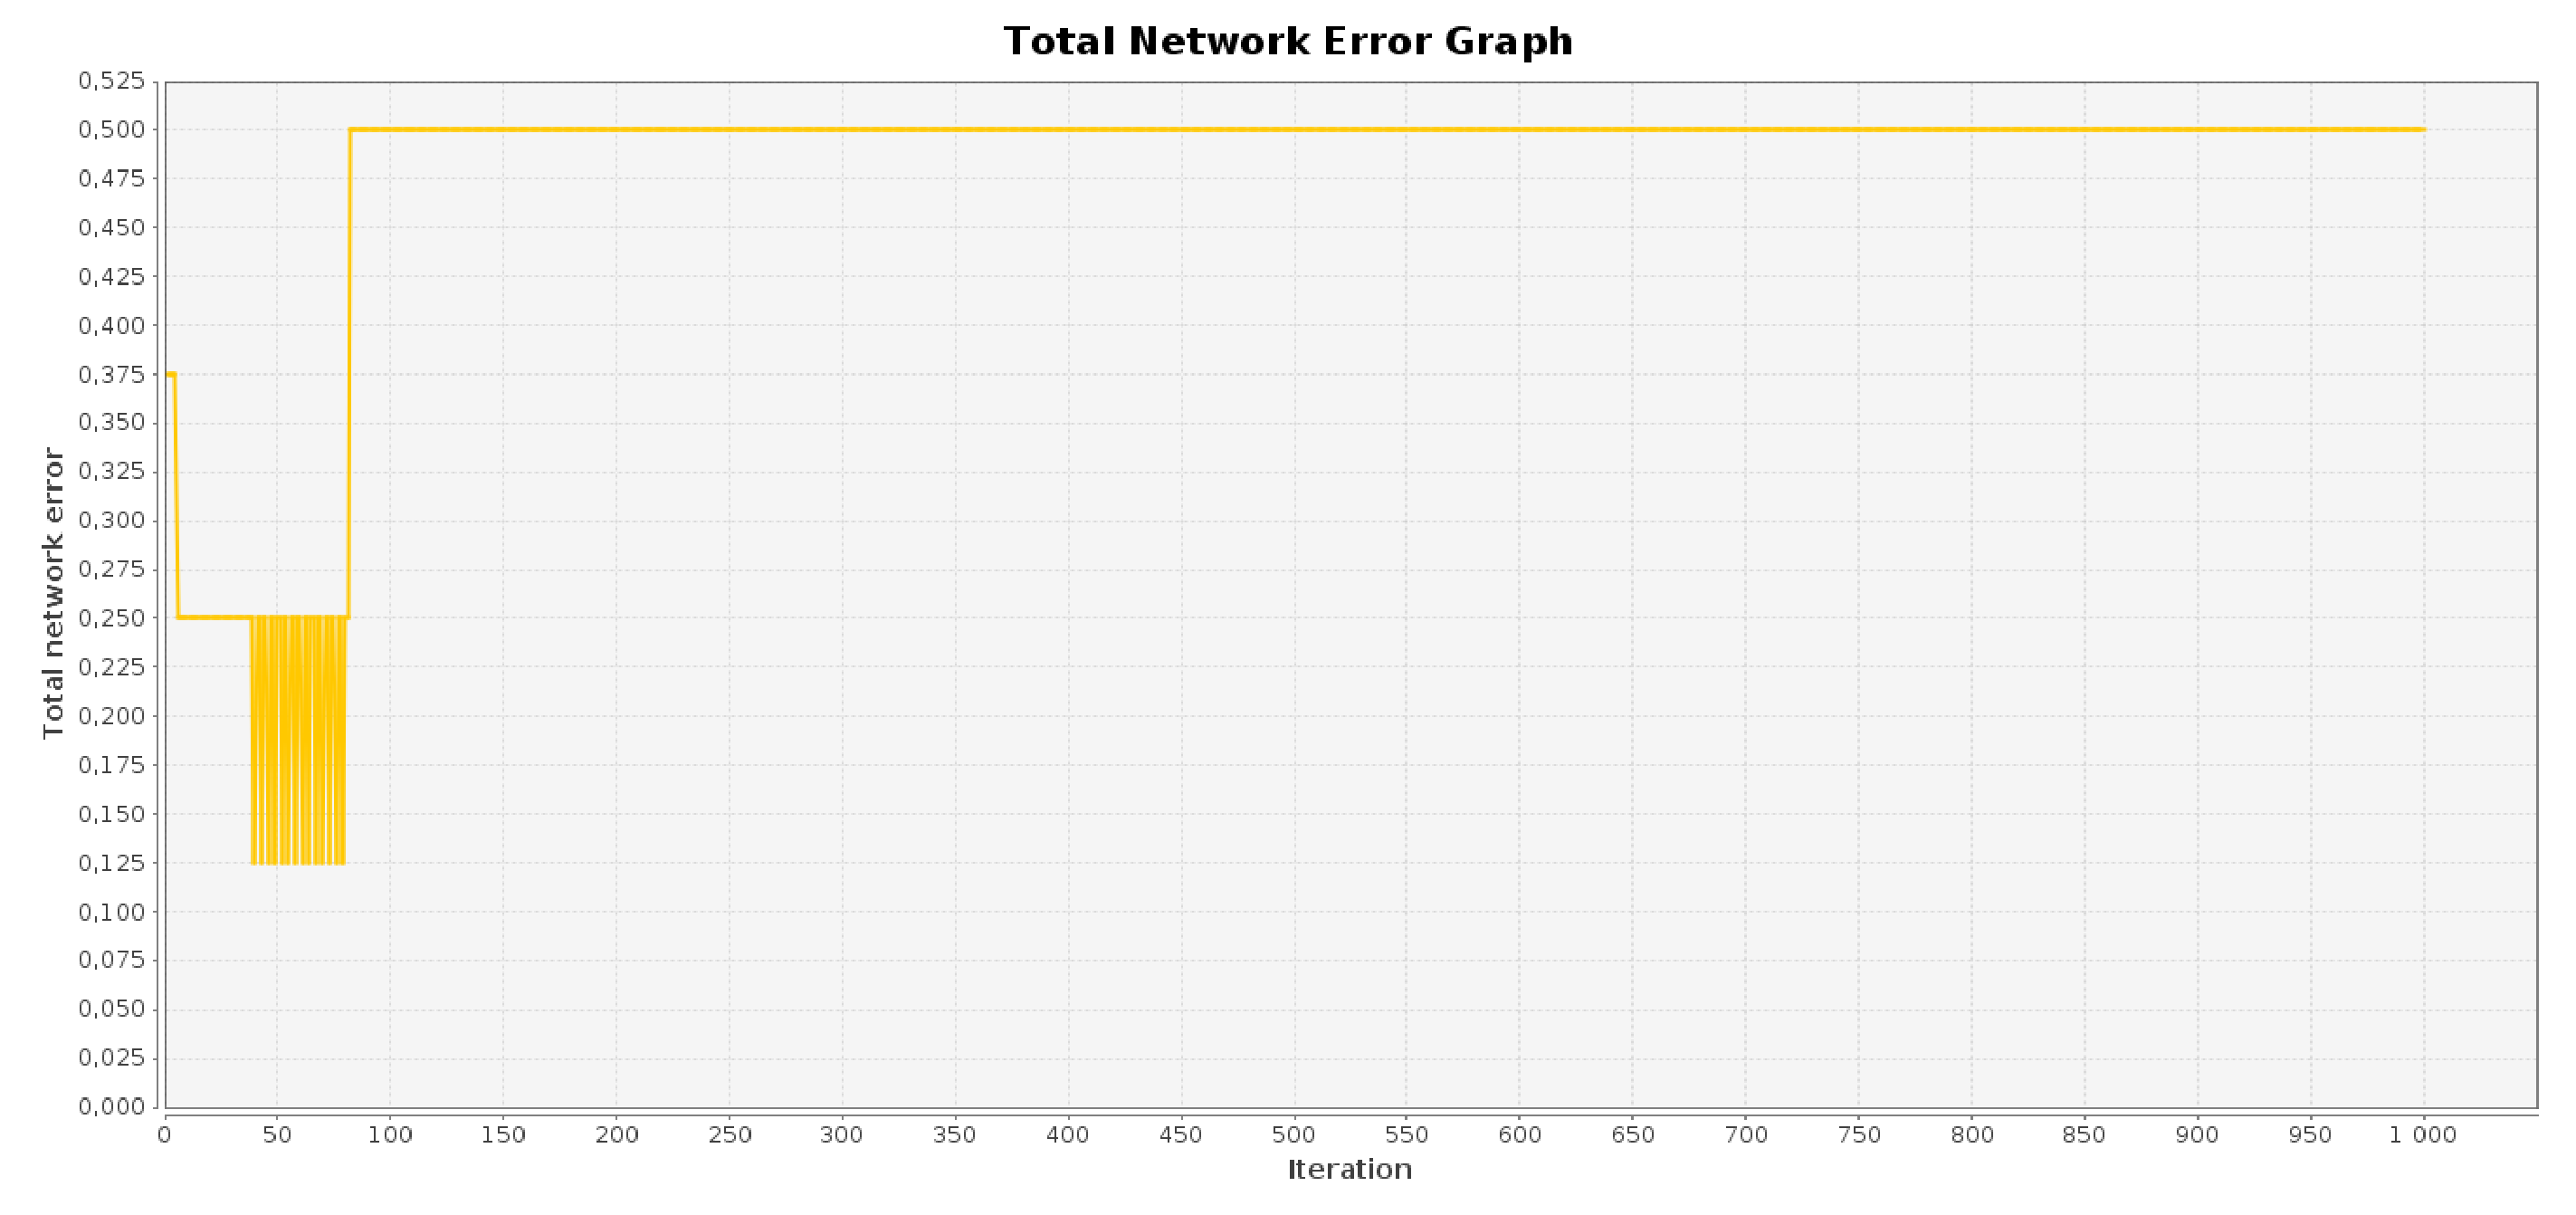
\includegraphics[width=6cm,height=3cm]{./pics/eq/mono_eq_0.01.eps}
\caption{Apprentissage fonction "et" avec un pas de 1}
\label{fig:anderr4}
\end{figure}

\begin{figure}[h]
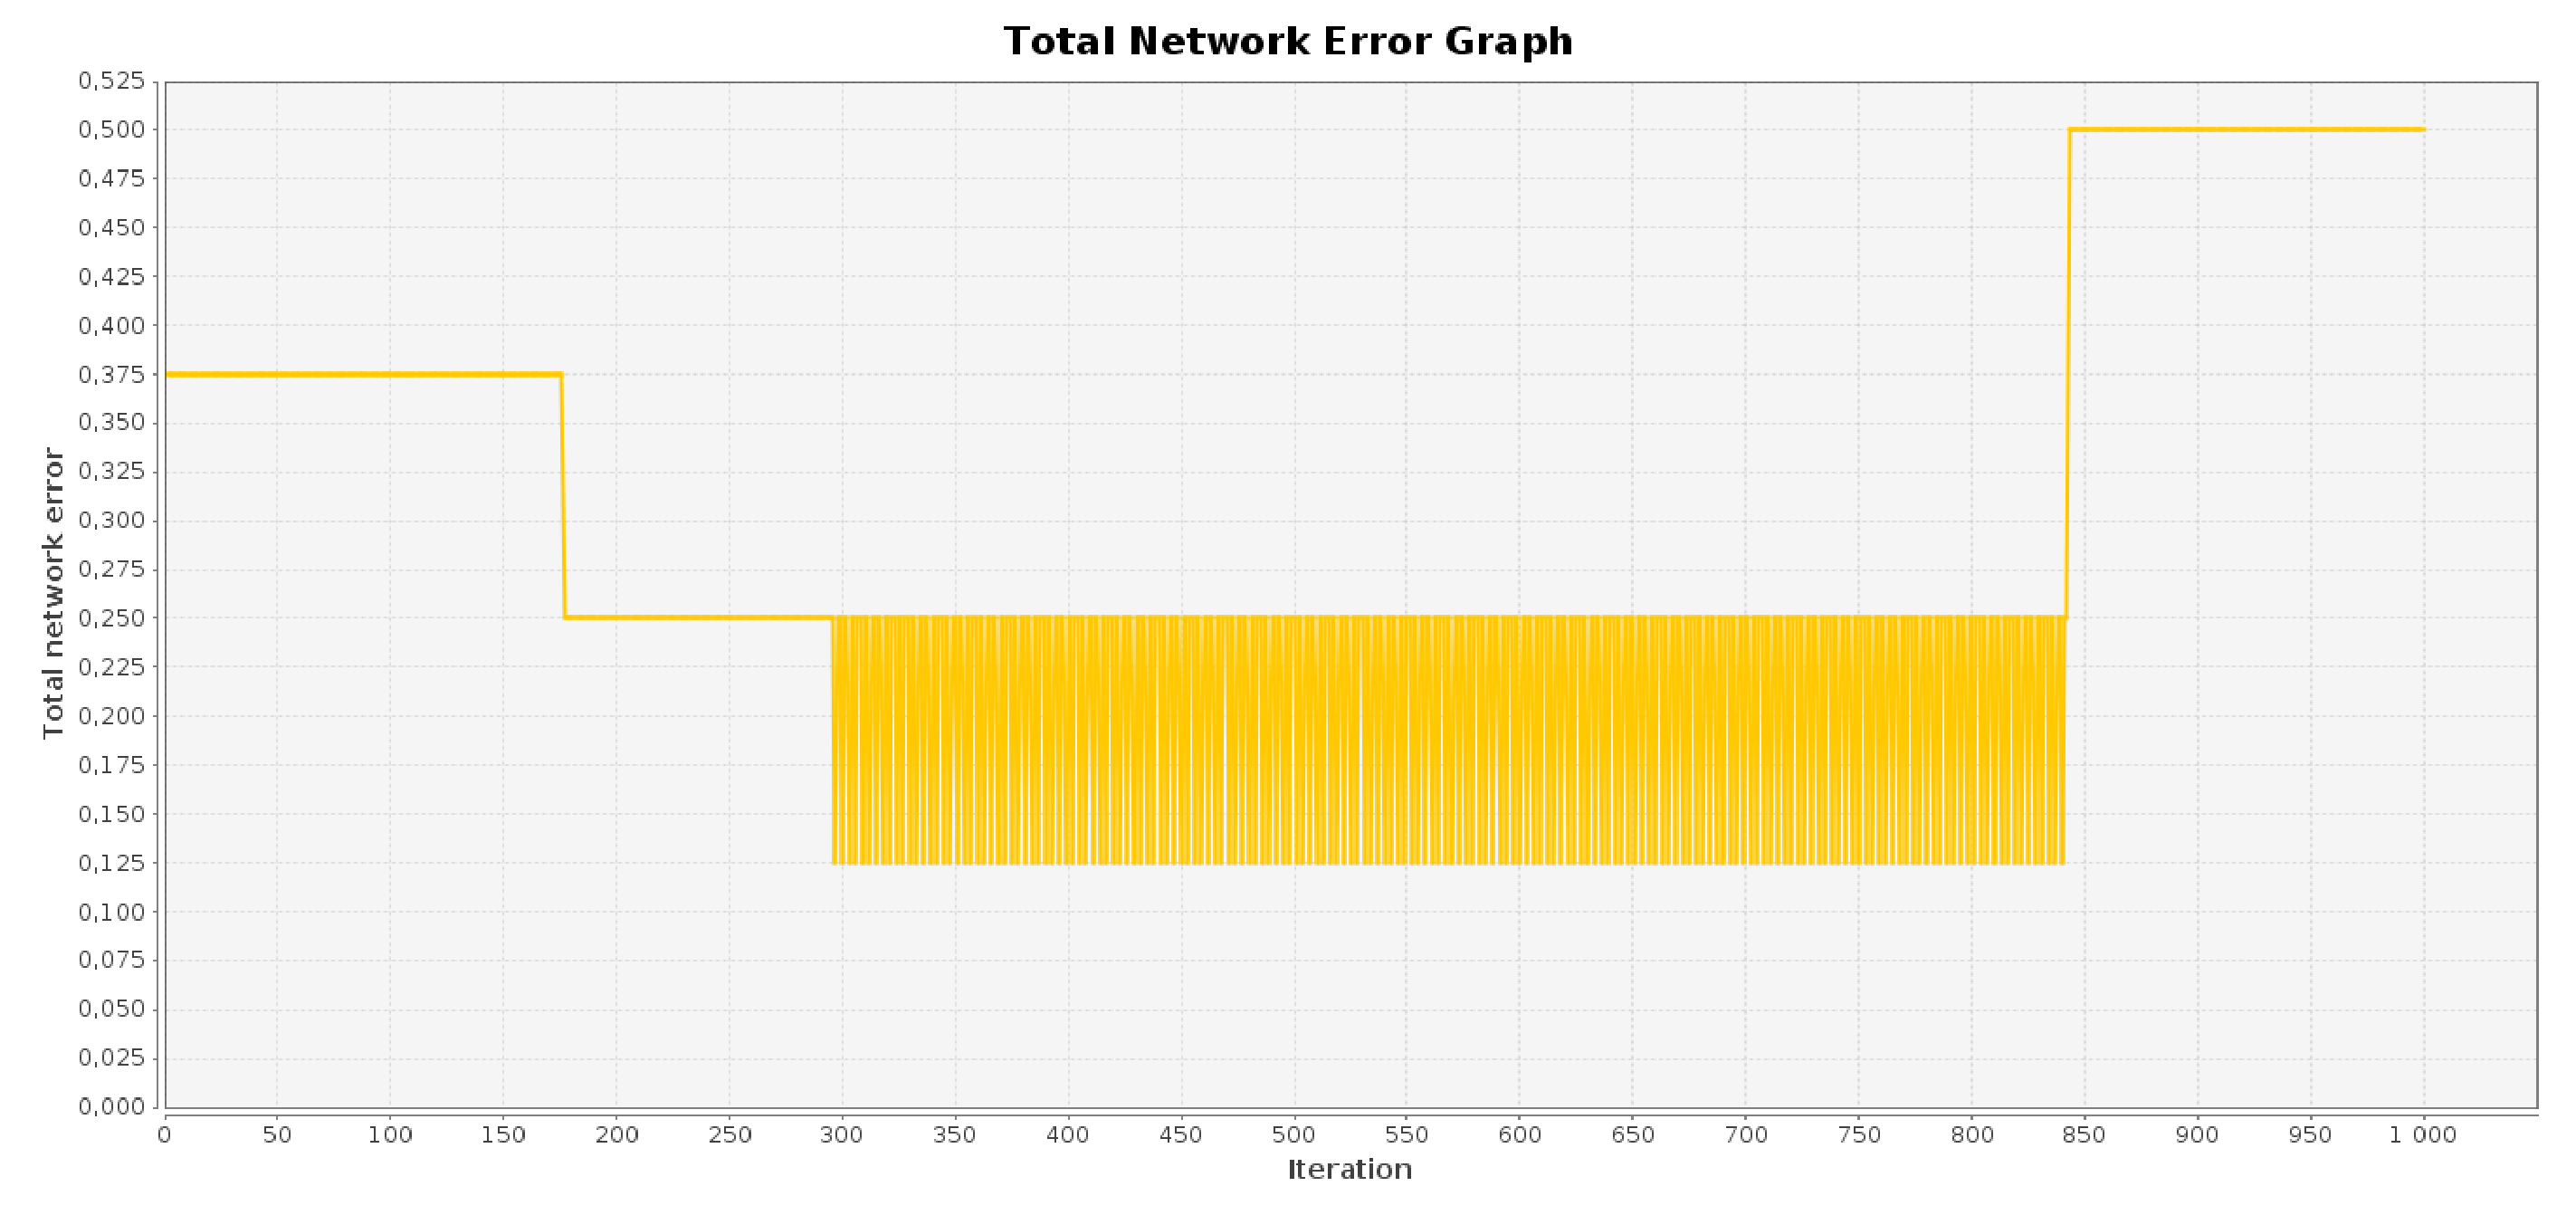
\includegraphics[width=6cm,height=3cm]{./pics/eq/mono_eq_0.001.eps}
\caption{Apprentissage fonction "et" avec un pas de 1}
\label{fig:anderr4}
\end{figure}

Nous pouvons encore observer que cela ne permet pas de conduire à une convergence.

Le perceptron monocouche ne semble donc pas adapté pour l'apprentissage de la fonction
d'équivalence. En effet, nous pouvons remarquer que l'équivalence n'est pas une fonction
linéairement séparable.

%TODO includegraphics{fonction non linéaire}

Ceci explique pourquoi un perceptron monocouche ne peut pas apprendre de manière correcte
la fonction d'équivalence.

\subsubsection{Un perceptron multicouche pour $ \Lefttrightarrow $}

Pour permettre l'apprentissage de l'équivalence par un perceptron, il faut donc que
celui-ci soit un perceptron multicouche.
Nous allons donc créer un perceptron multicouche qui contiendra une couche caché de
3 neurones, et avec toujours 2 inputs et un un output.
Cela nous donne le perceptron ci-dessous:

\begin{figure}[h]
\centering
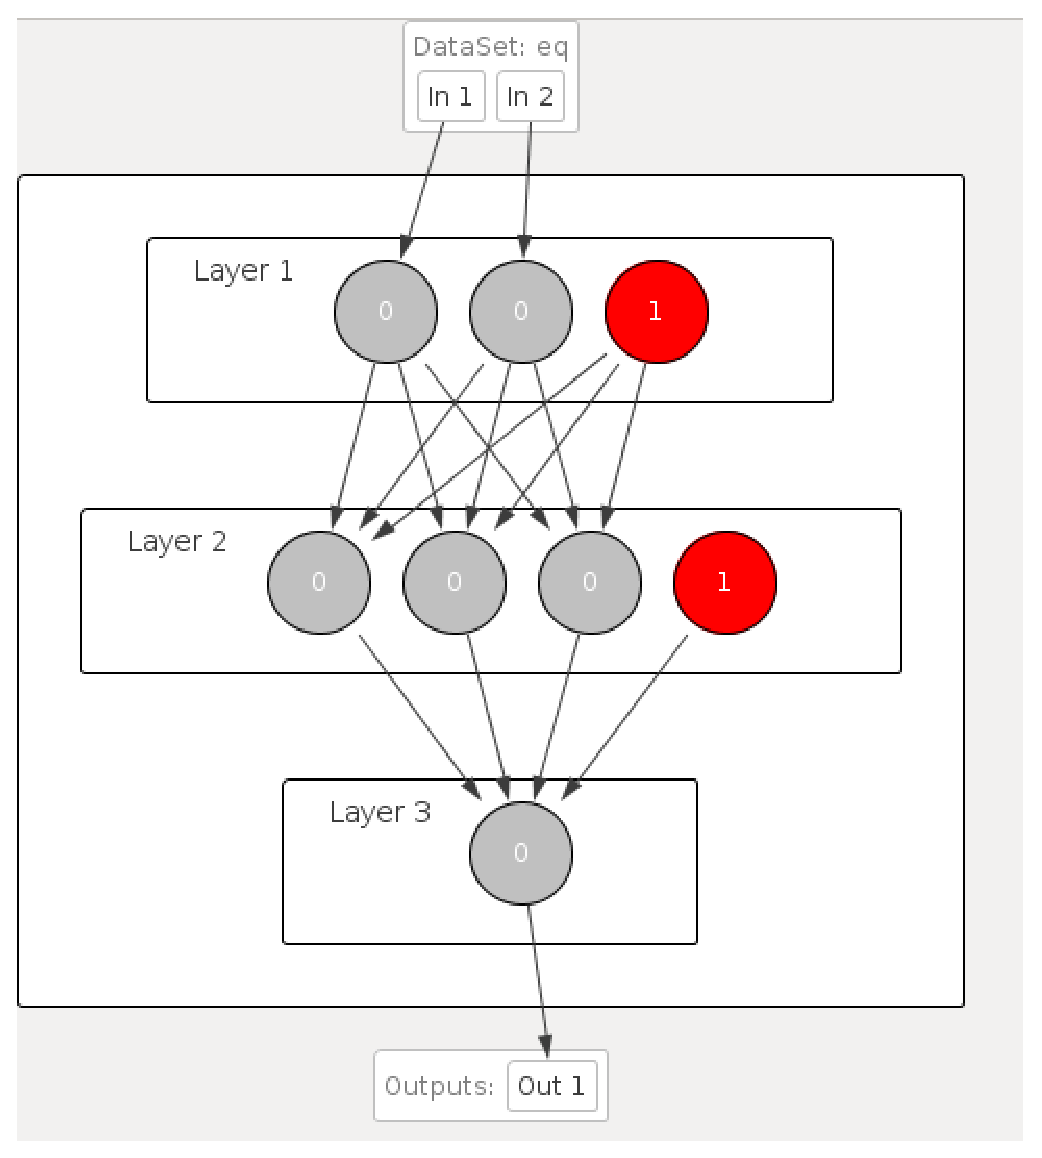
\includegraphics[width=5cm,height=7cm]{./pics/eq/perceptron_multi.eps}
\caption{Apprentissage fonction "et" avec un pas de 1}
\label{fig:anderr4}
\end{figure}

Testons ce perceptron avec le data set et les paramètre par défaut.

\begin{figure}[h]
\centering
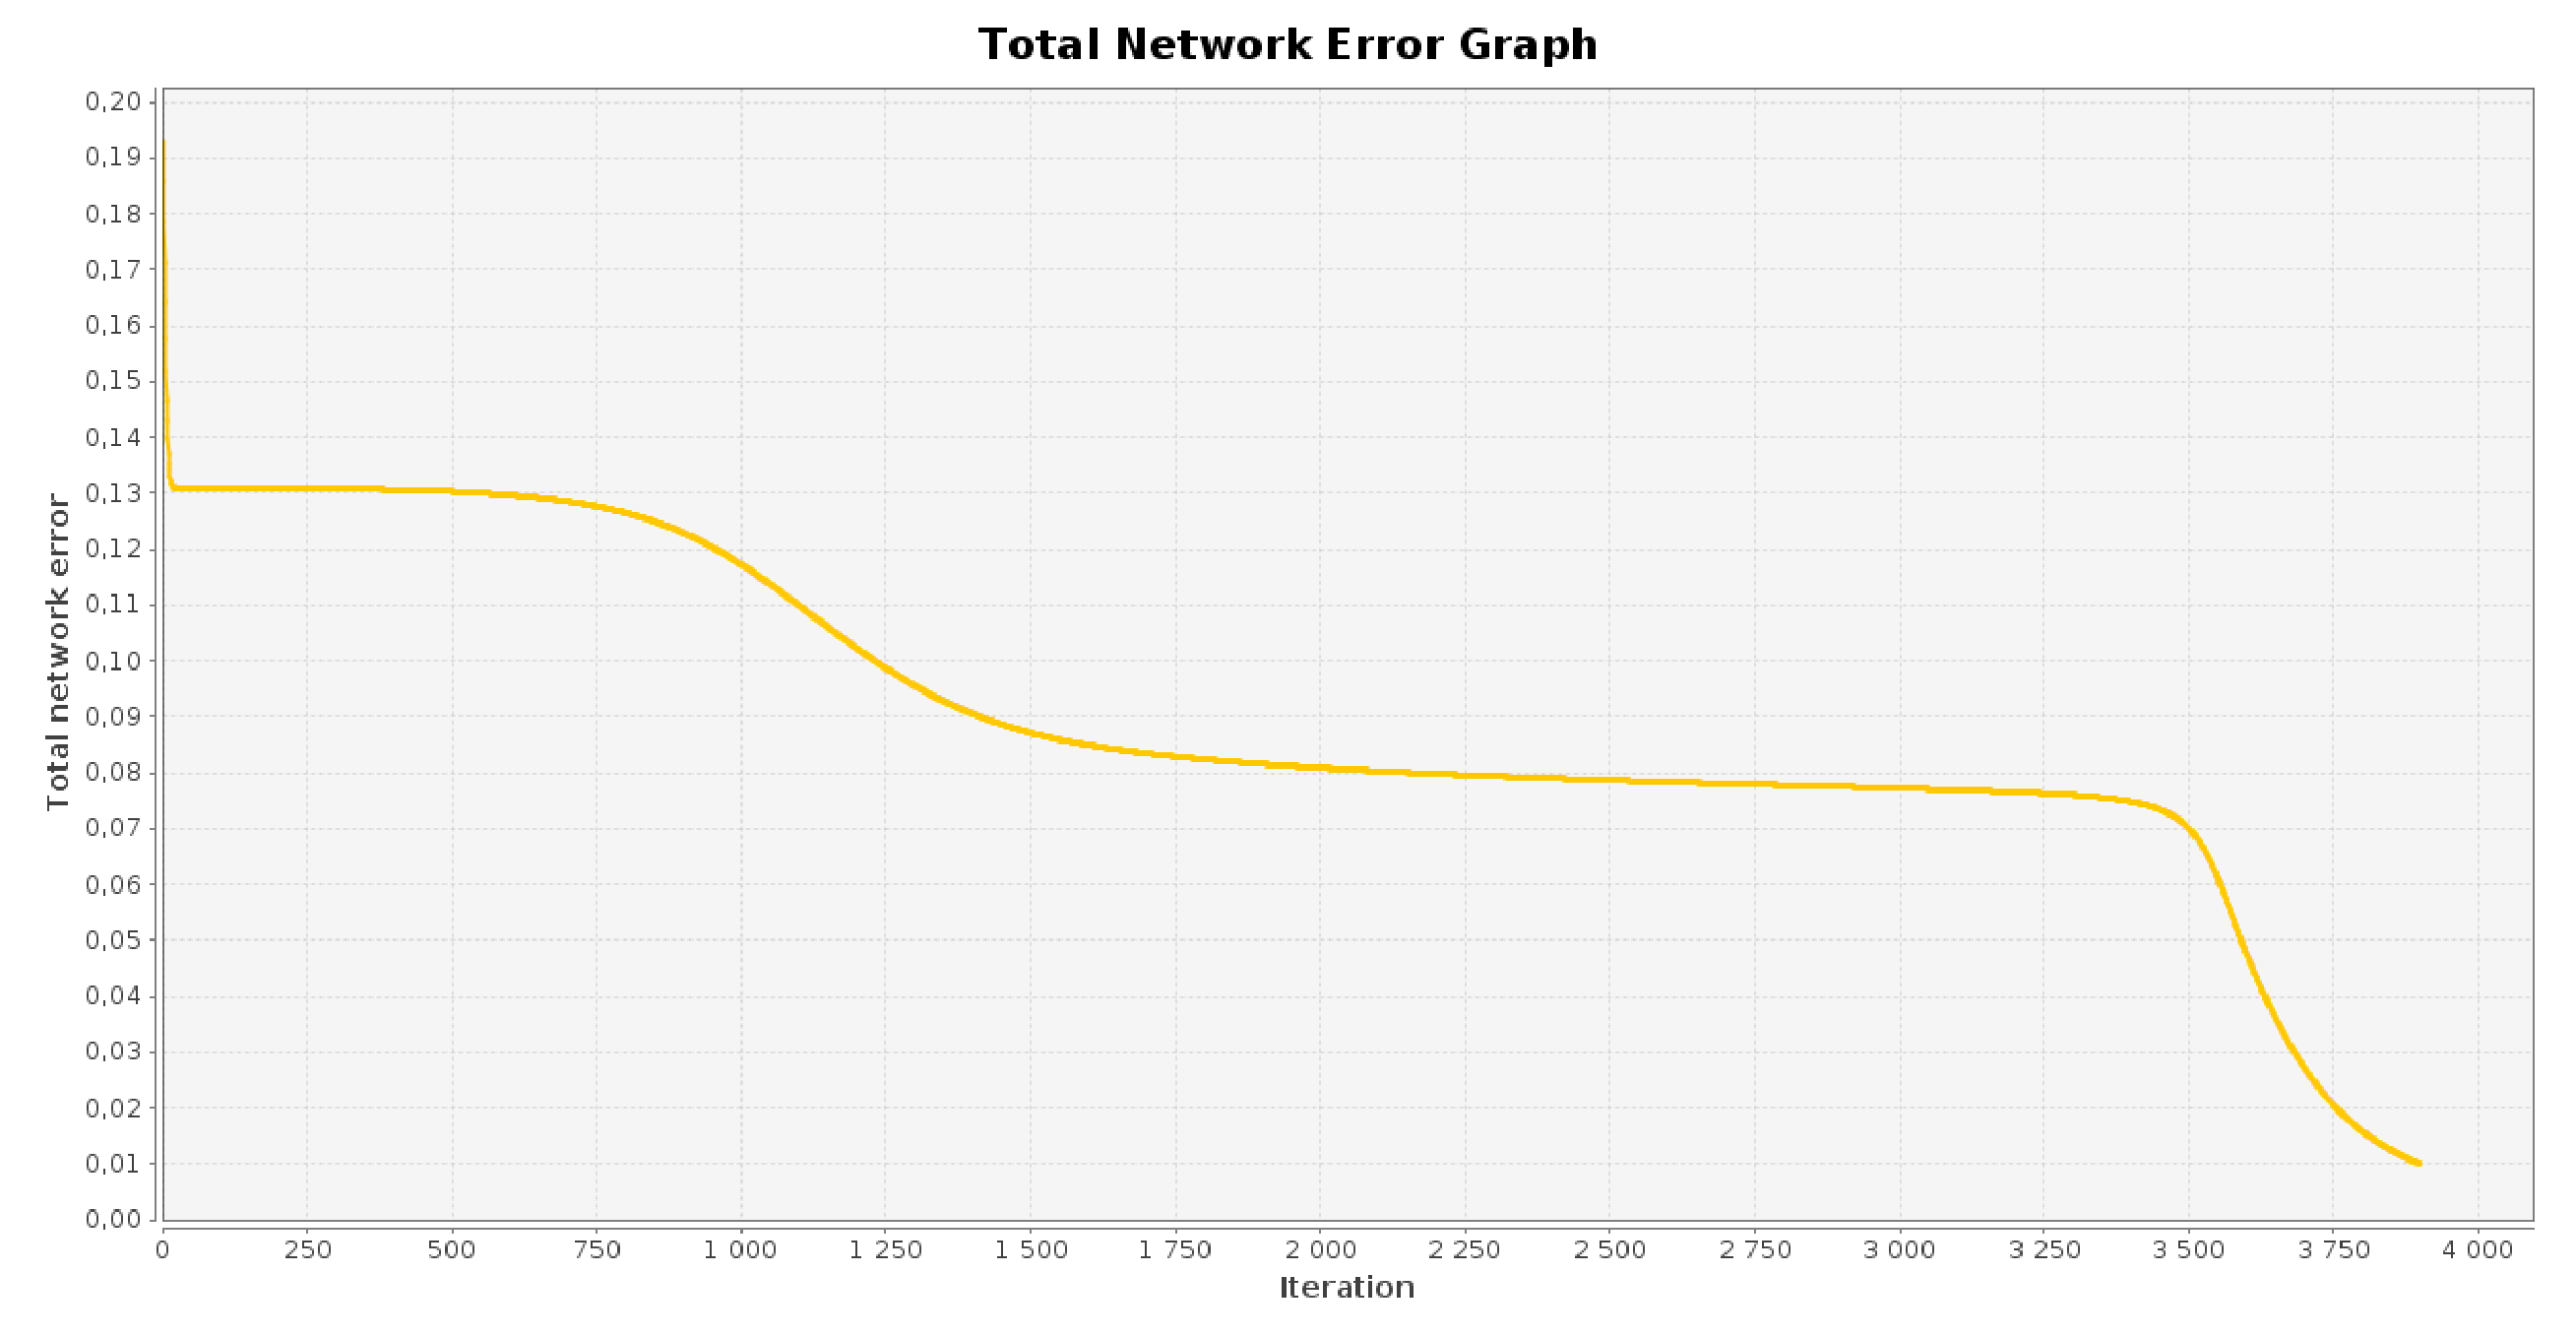
\includegraphics[width=12cm,height=9cm]{./pics/eq/multi_eq_def.eps}
\caption{Apprentissage fonction "et" avec un pas de 1}
\label{fig:anderr4}
\end{figure}

Il semble y avoir une convergence vers 3900 itérations.

Nous allons maintenant voir l'influence des paramètre sur la courbe. Voyons tout d'abord
les effets d'un changement de pas d'apprentissage.

Les pas d'apprentissages sont respectivement de 0.1 , 0.5 , 1.

\begin{figure}[h]
\caption{Apprentissage fonction "et" avec un pas de 1}
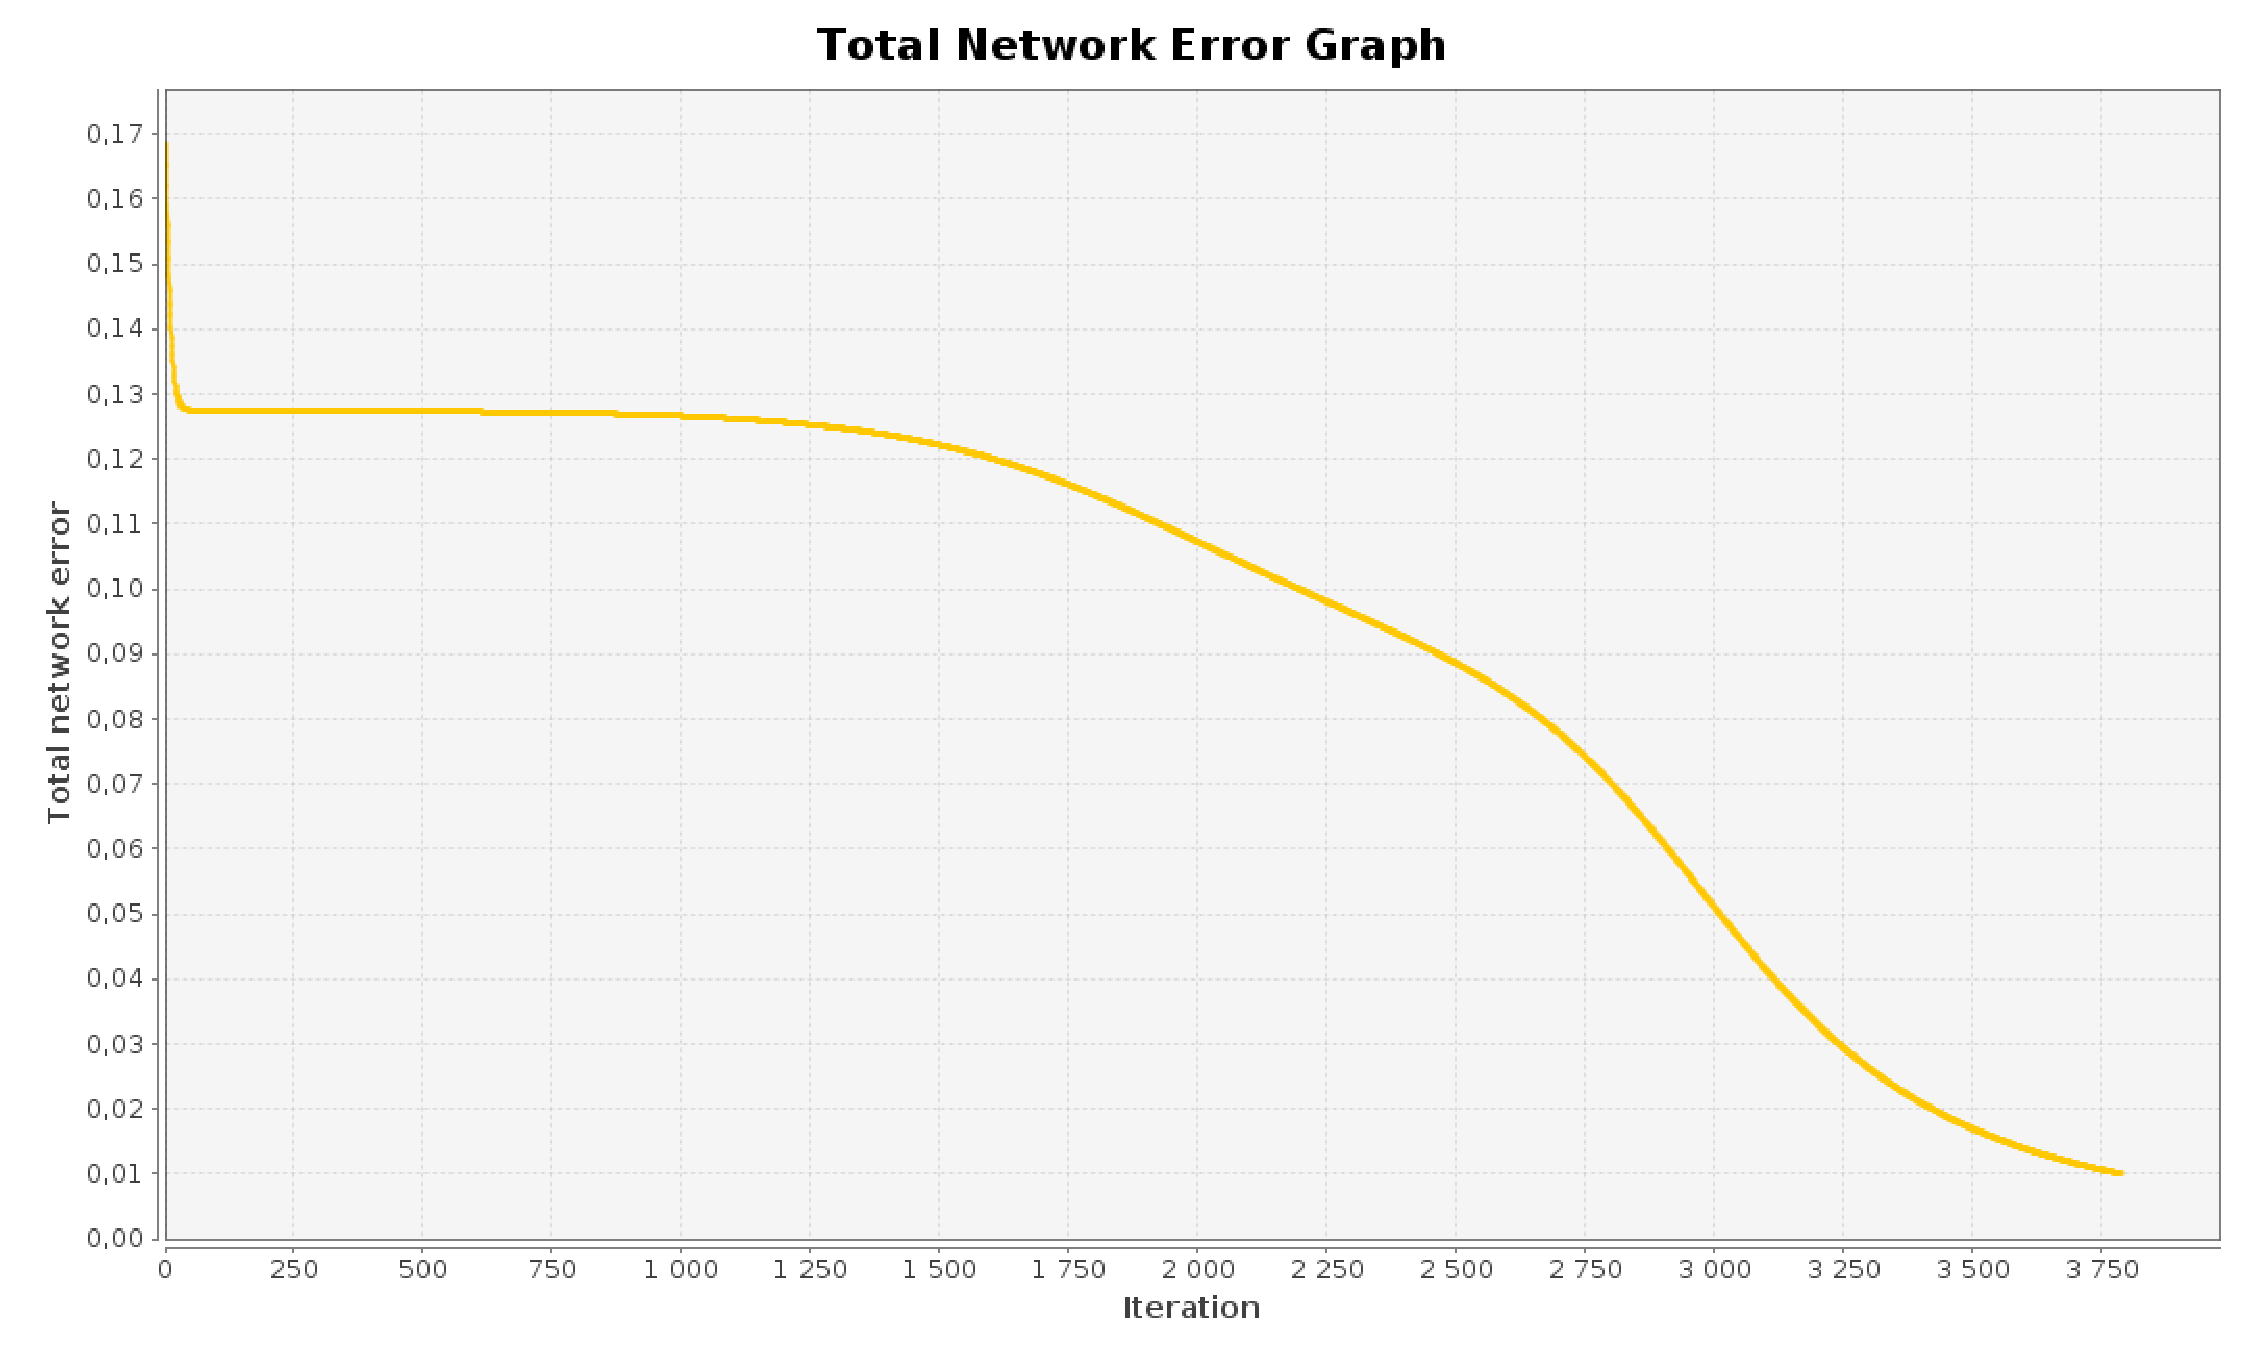
\includegraphics[width=6cm,height=3cm]{./pics/eq/multi_eq_0.1.eps}
\label{fig:anderr4}
\end{figure}

\begin{figure}[h]
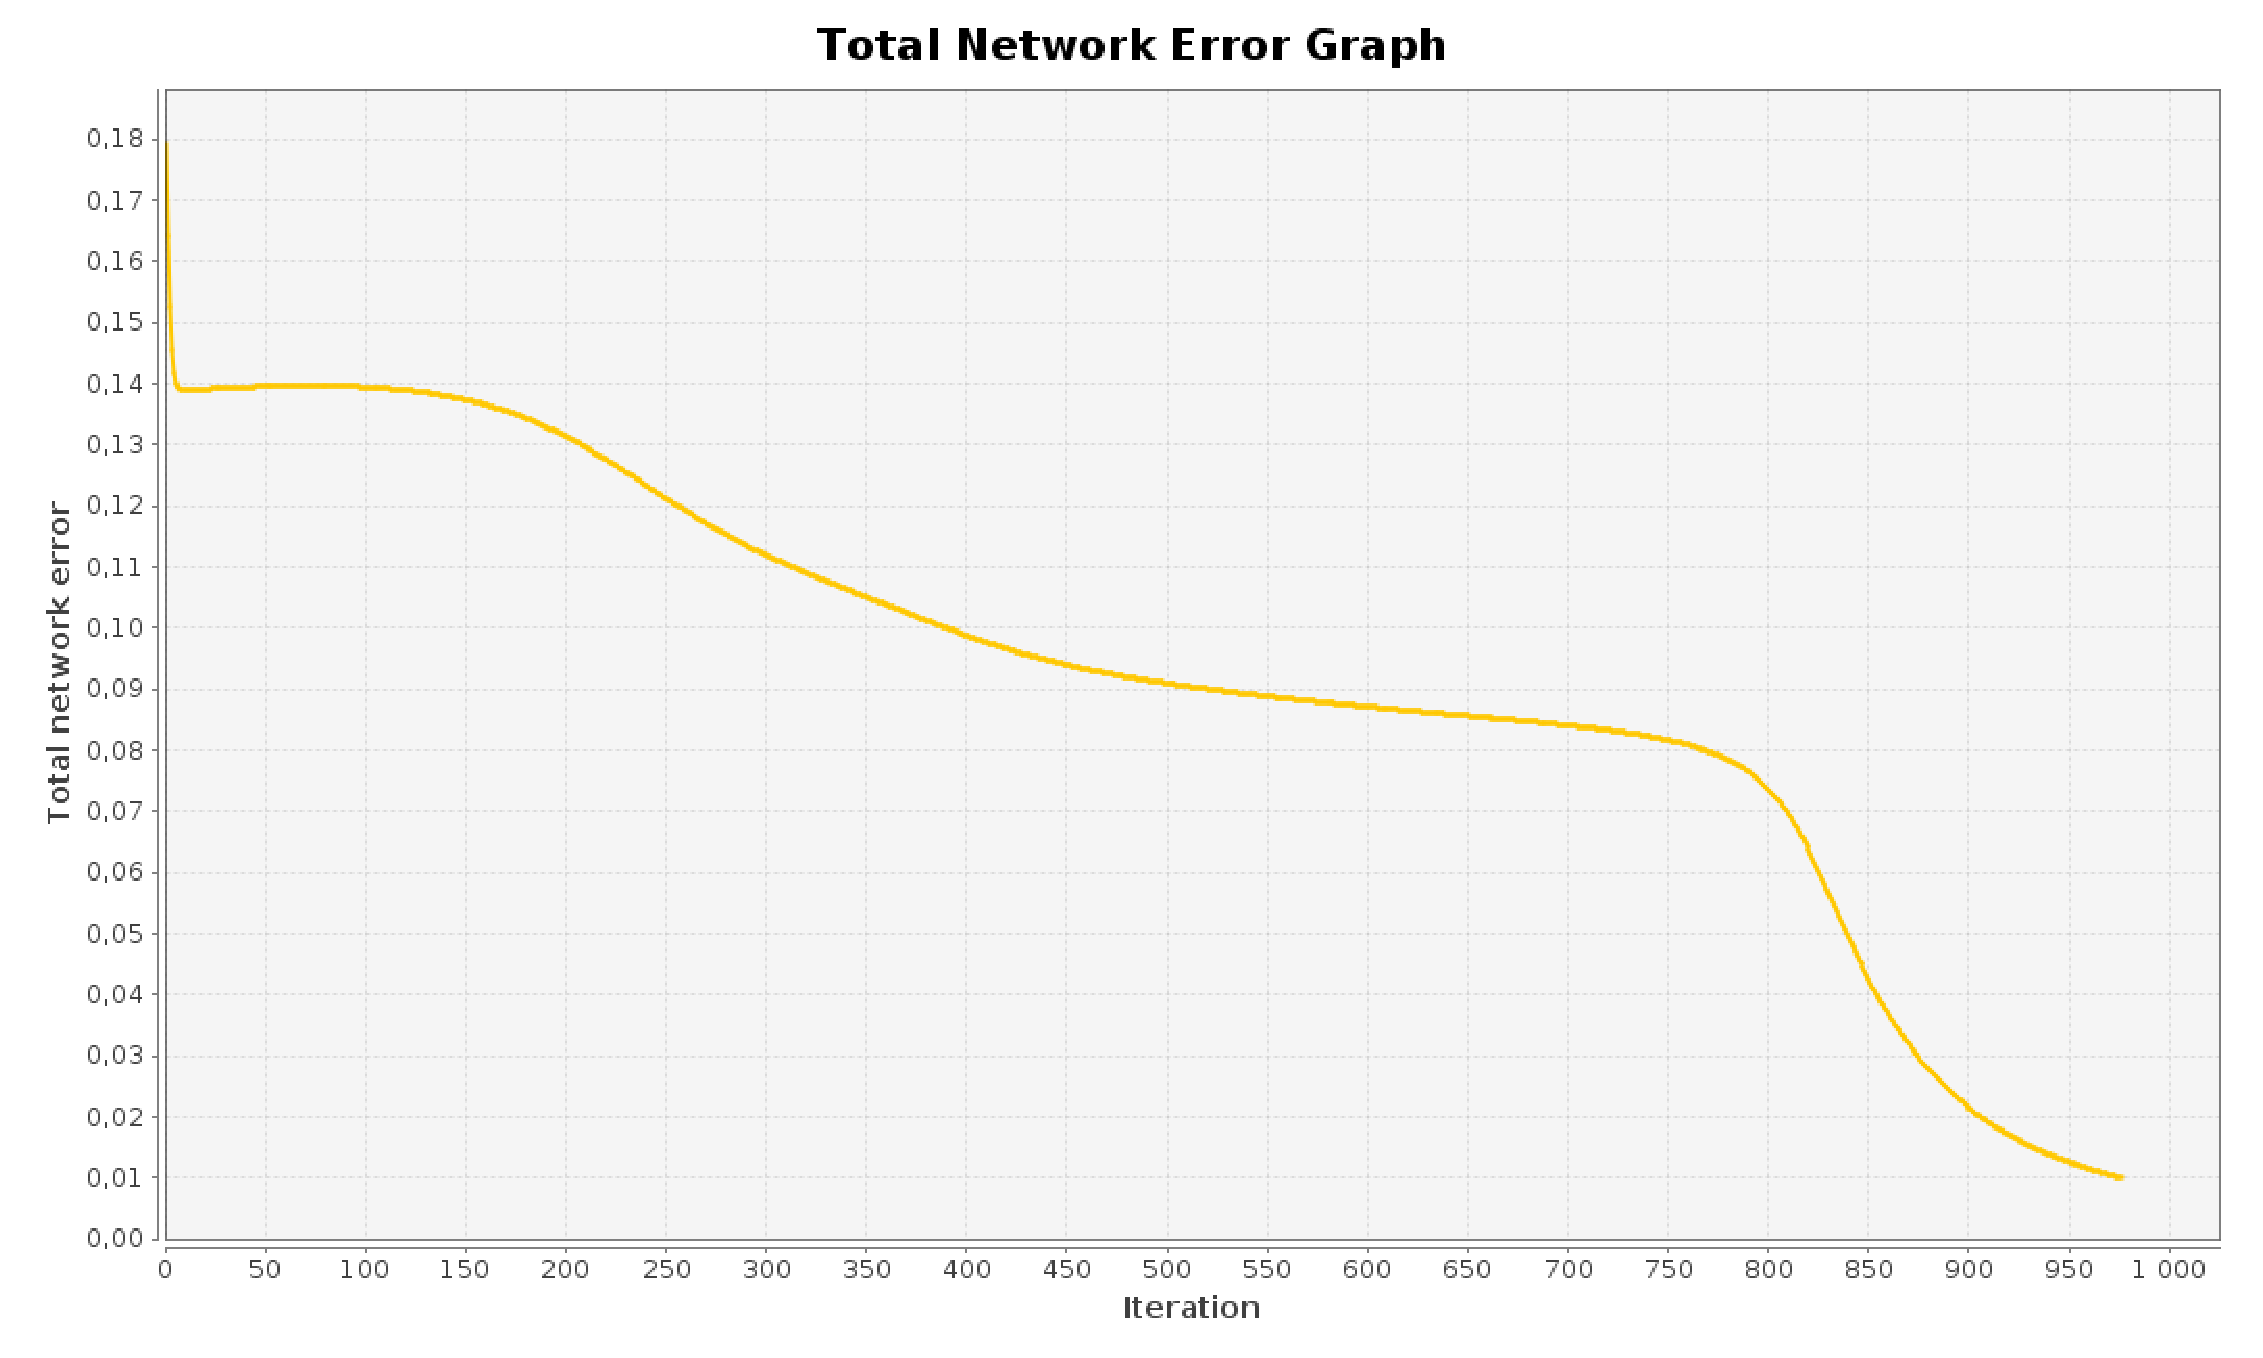
\includegraphics[width=6cm,height=3cm]{./pics/eq/multi_eq_0.5.eps}
\caption{Apprentissage fonction "et" avec un pas de 1}
\label{fig:anderr4}
\end{figure}

\begin{figure}[h]
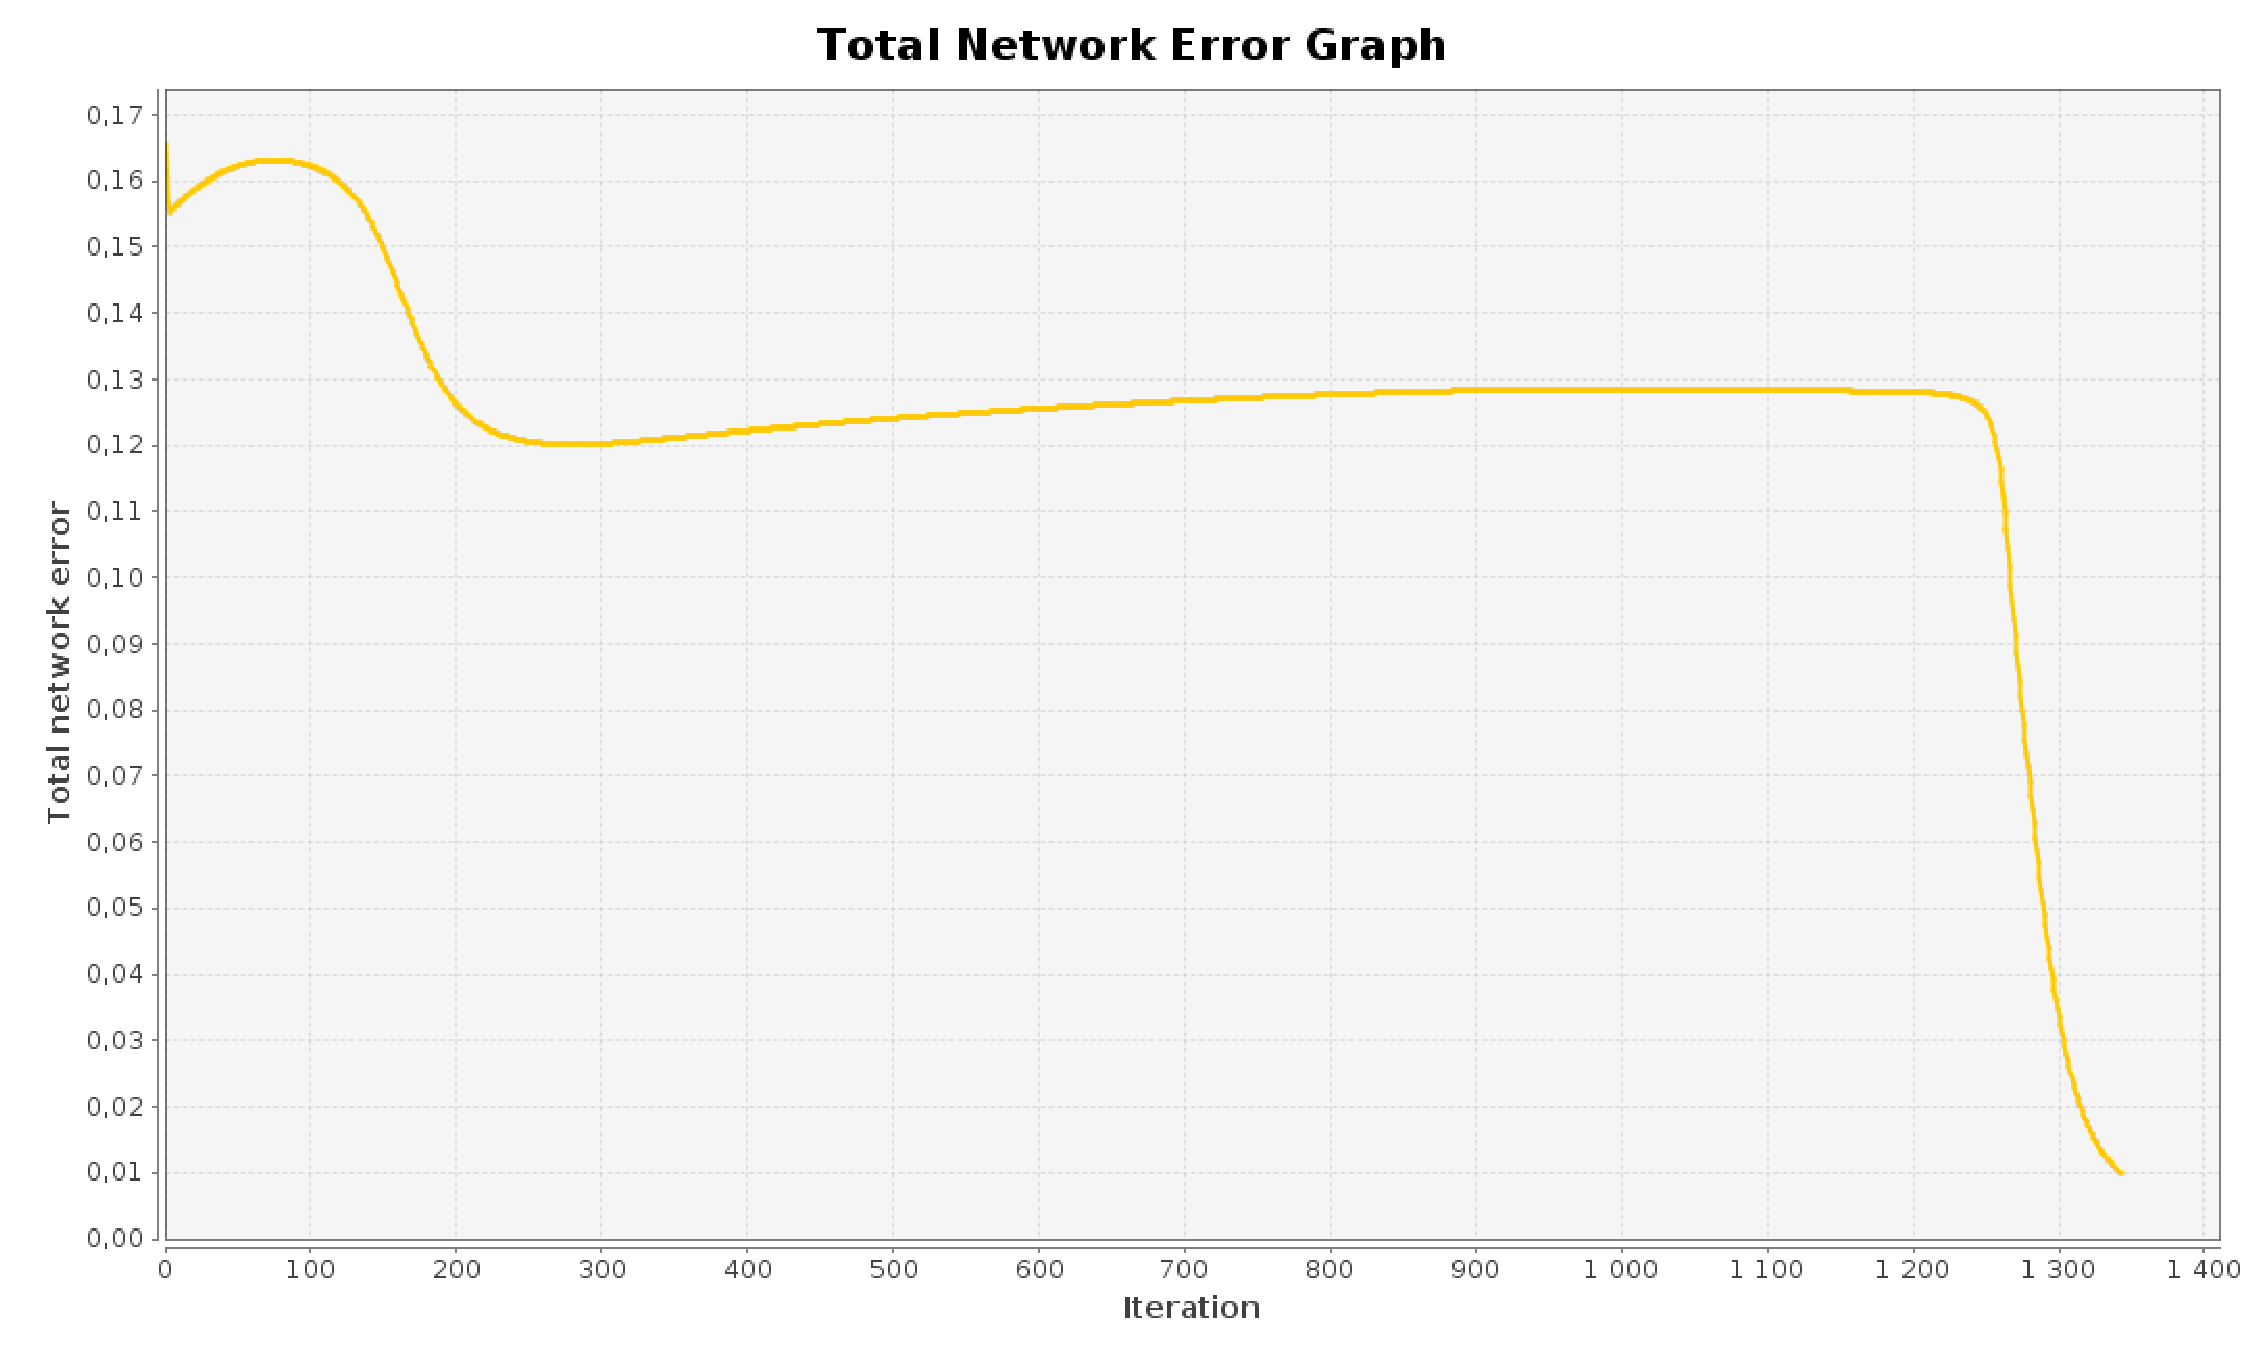
\includegraphics[width=6cm,height=3cm]{./pics/eq/multi_eq_1.eps}
\caption{Apprentissage fonction "et" avec un pas de 1}
\label{fig:anderr4}
\end{figure}

Changeons à présent le nombre de neurone dans la couche caché.
Nous allons partir d'un réseau de 5 neurones, et le doublé d'un perceptron
à l'autre. Nous pourrons ainsi voir assez rapidement si le nombre de neurone
influe grandement sur les résultats.
Les graphique représente donc respectivement les résultats pour
des perceptrons de 5, 10 et 20 neurone dans une couche caché.

\begin{figure}[h]
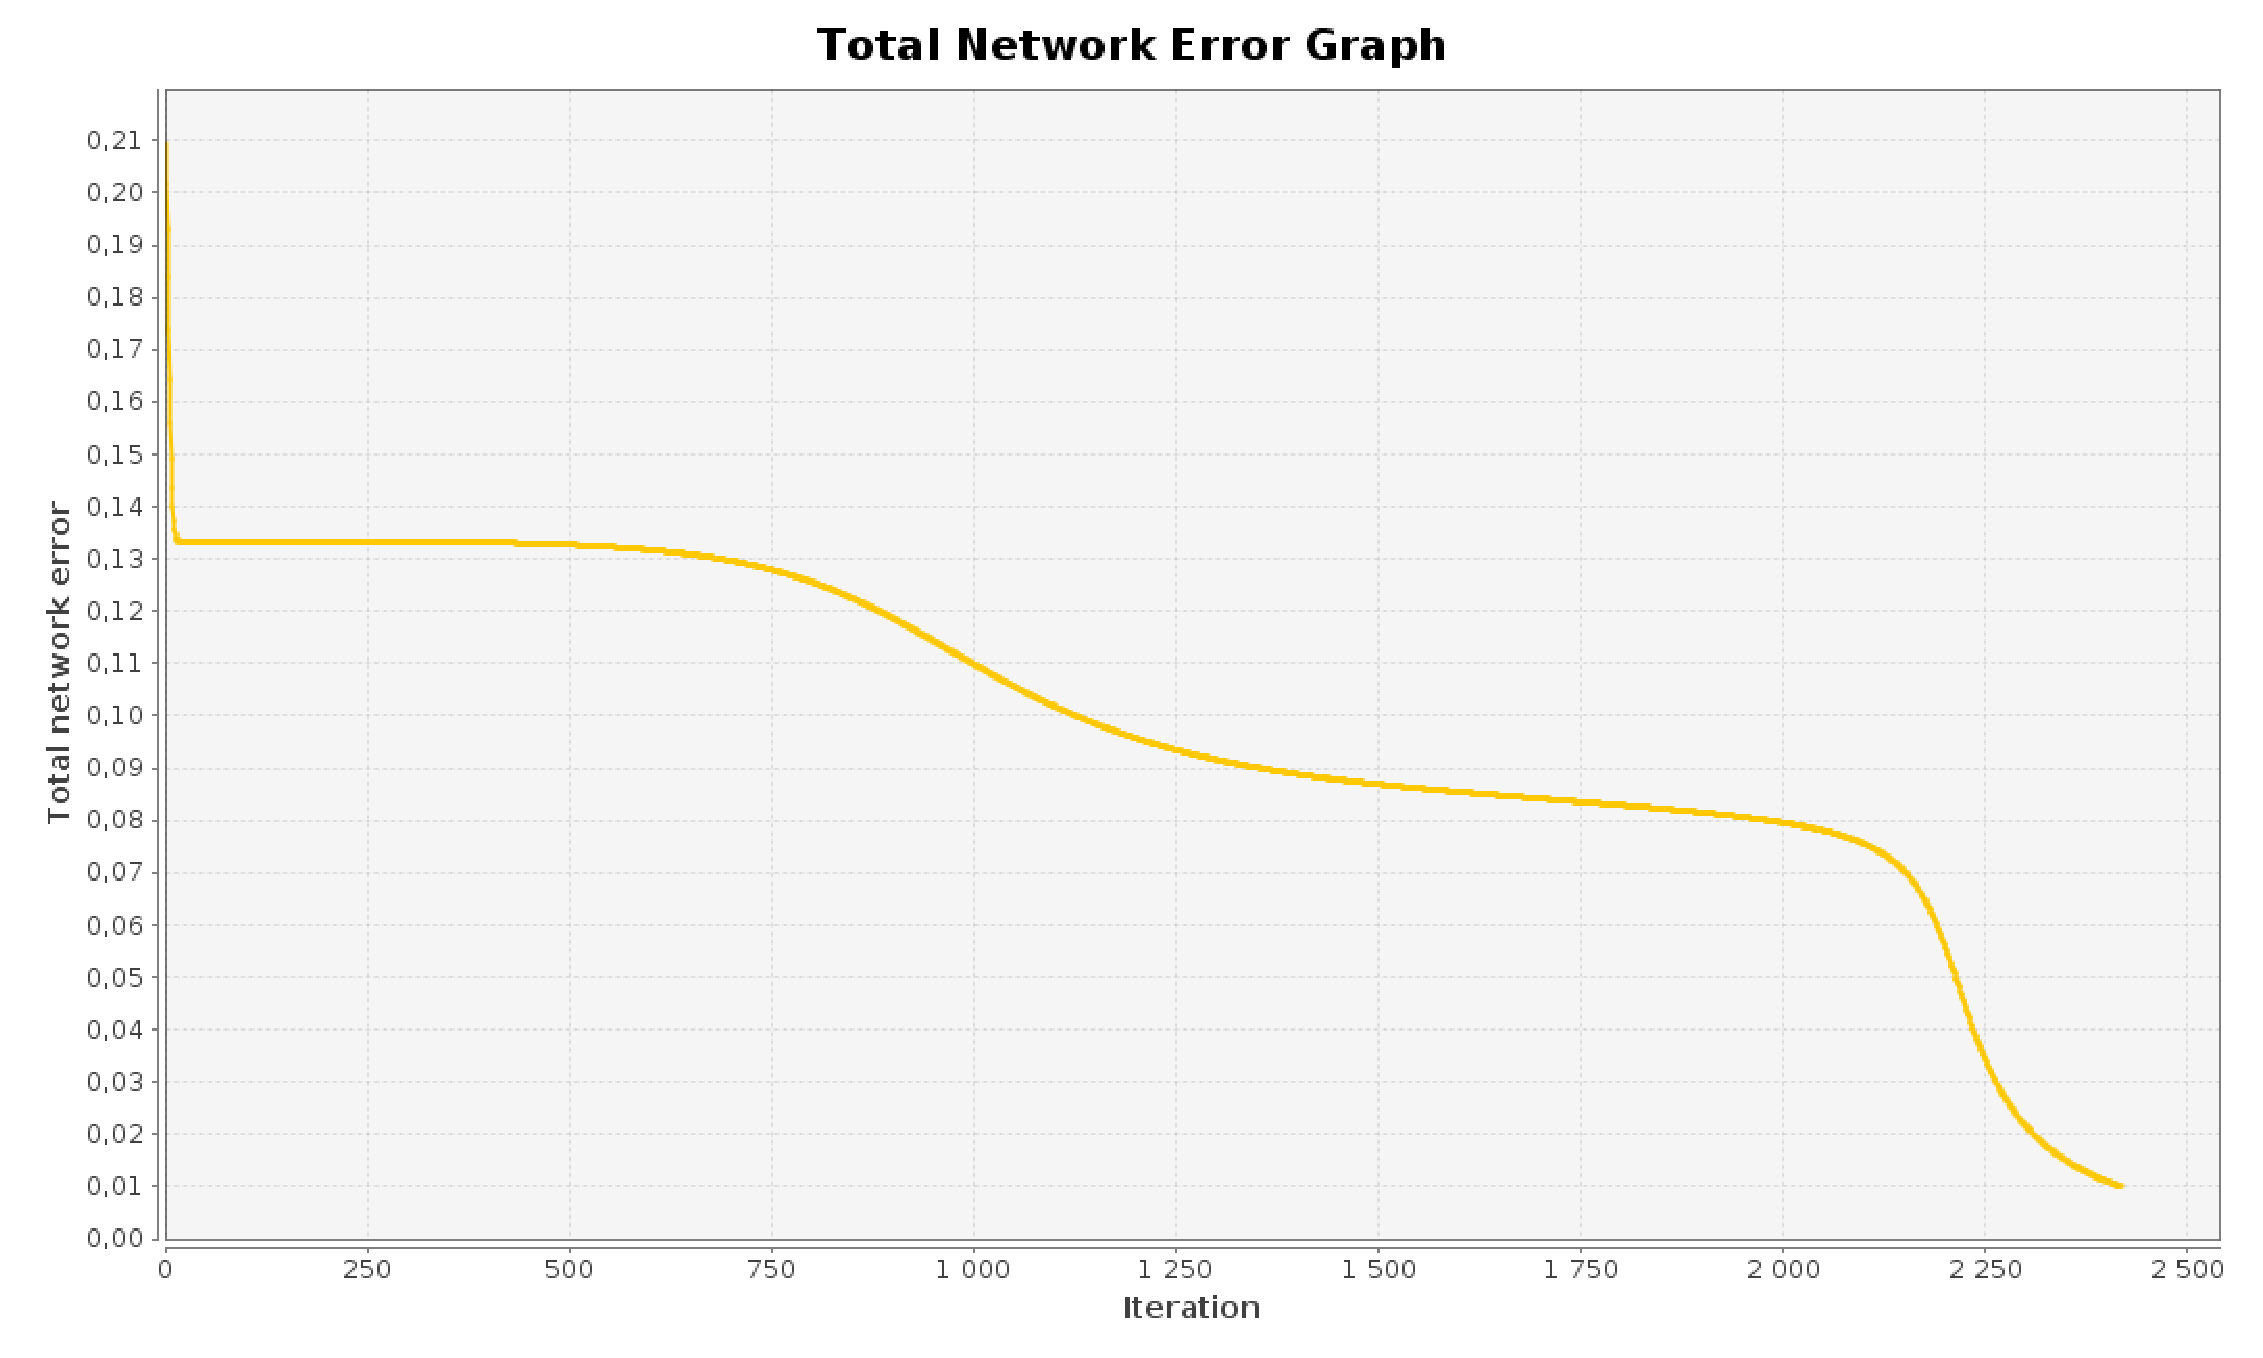
\includegraphics[width=6cm,height=3cm]{./pics/eq/multi-5_eq_def.eps}
\caption{Apprentissage fonction "et" avec un pas de 1}
\label{fig:anderr4}
\end{figure}

\begin{figure}[h]
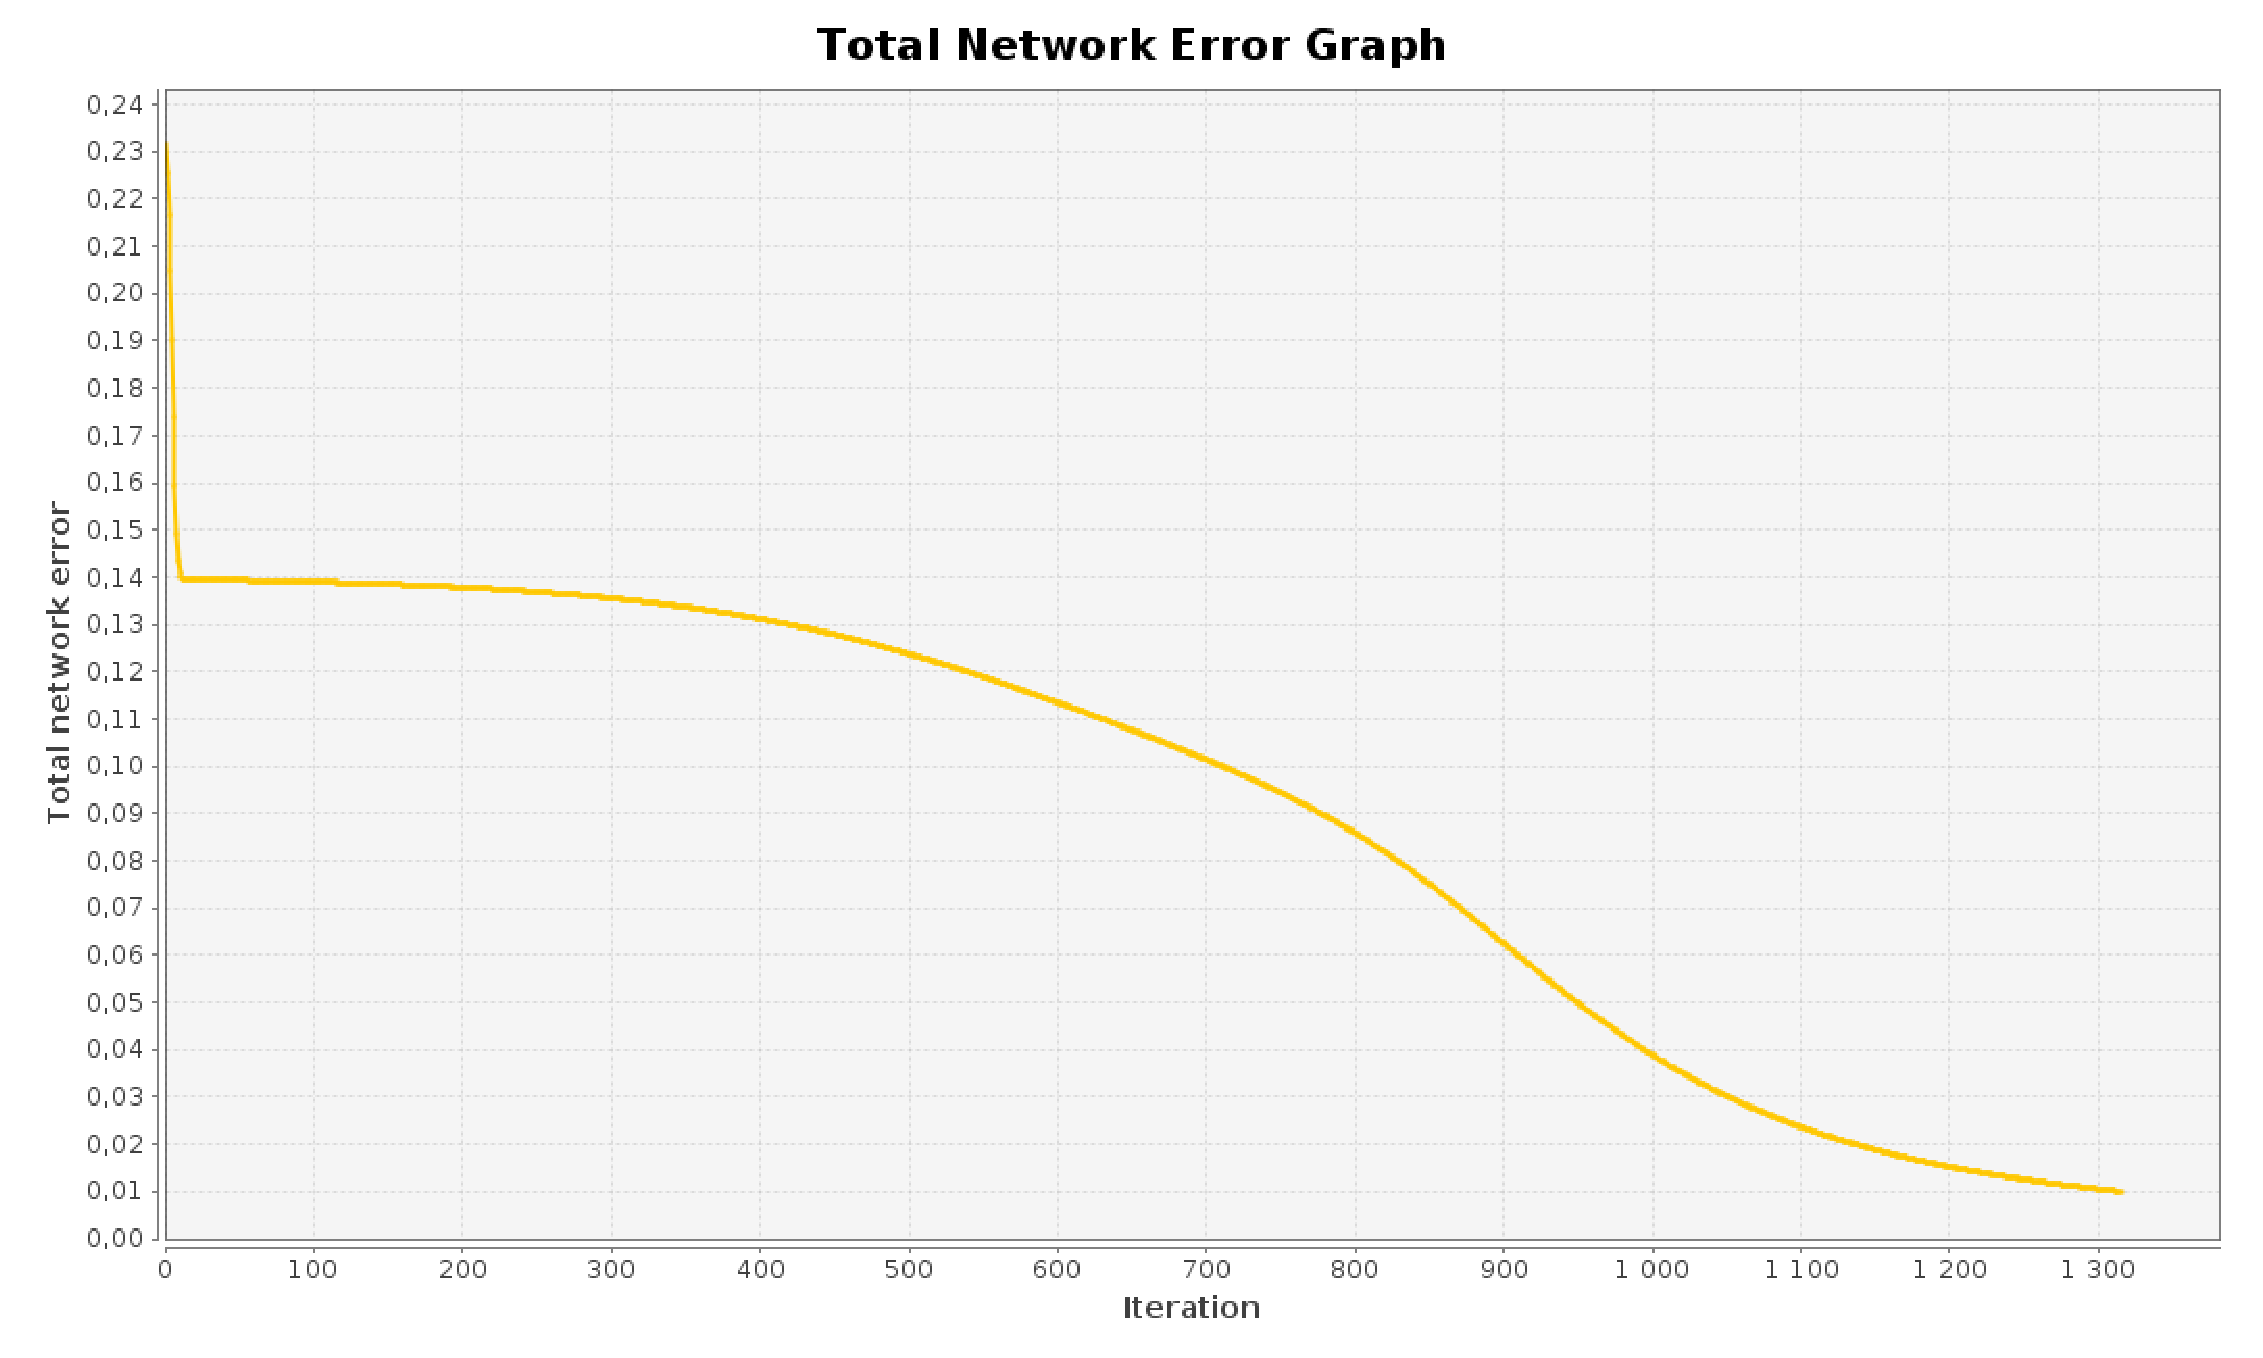
\includegraphics[width=6cm,height=3cm]{./pics/eq/multi-10_eq_def.eps}
\caption{Apprentissage fonction "et" avec un pas de 1}
\label{fig:anderr4}
\end{figure}

\begin{figure}[h]
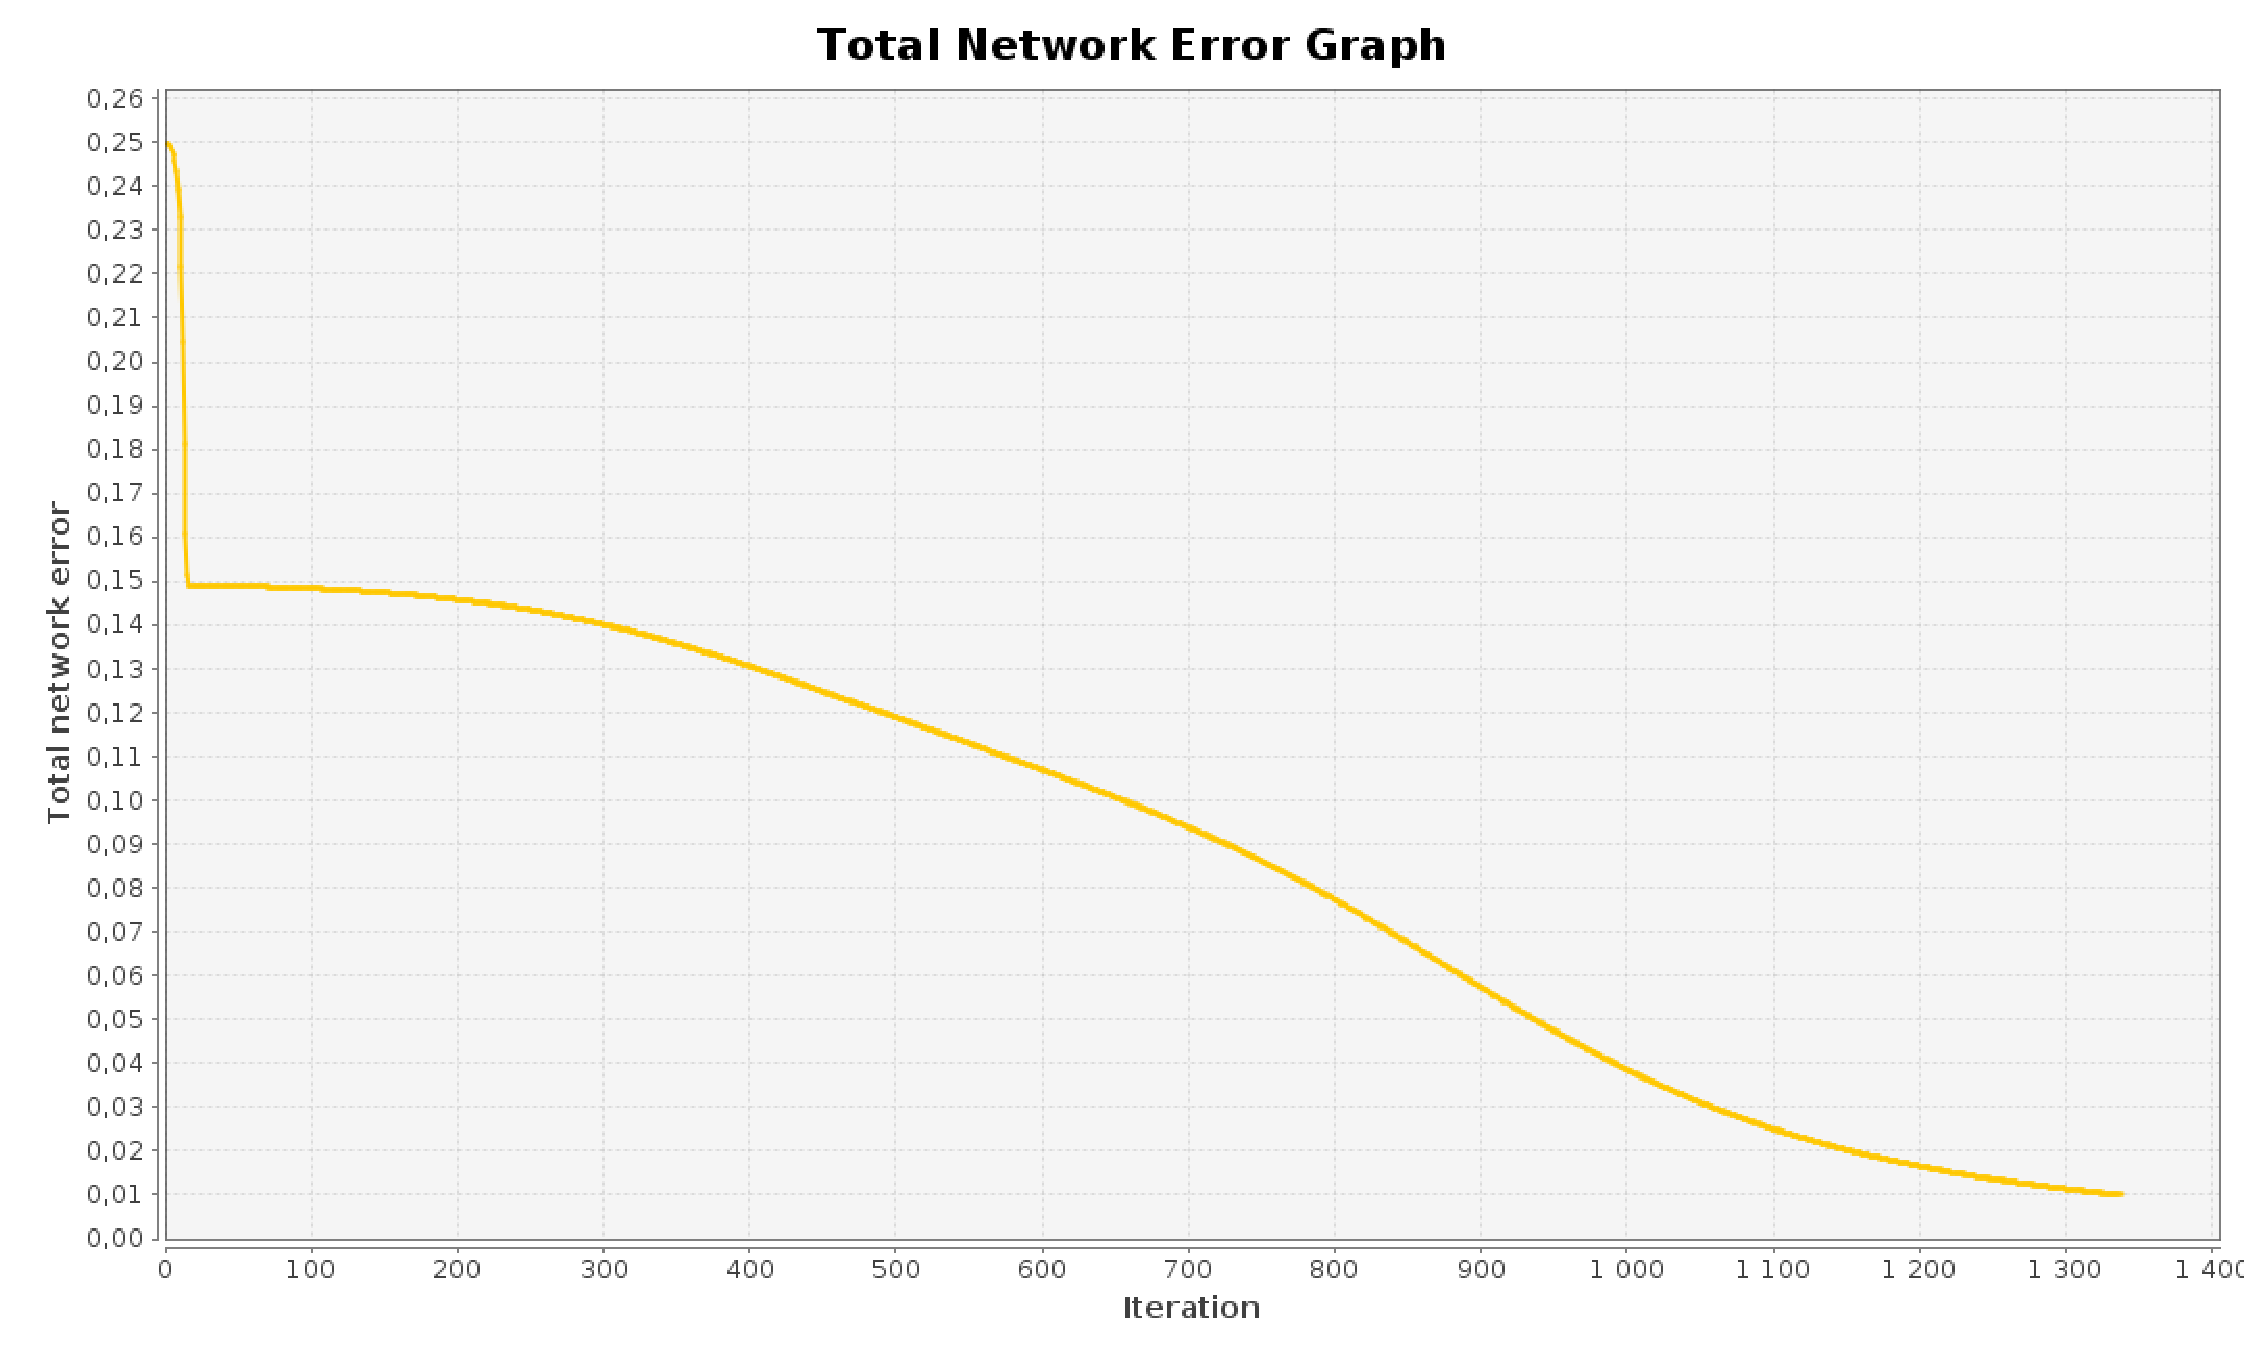
\includegraphics[width=6cm,height=3cm]{./pics/eq/multi-20_eq_def.eps}
\caption{Apprentissage fonction "et" avec un pas de 1}
\label{fig:anderr4}
\end{figure}


Augmenter le nombre neurone dans la couche caché semble diminuer le nombre
d'itération nécessaire pour que la courbe converge.
La courbe semble aussi être plus "lisse".

Essayons maintenant maintenant d'ajouter plus de couche cachées. Voyons la
courbe que l'on obtient avec un perceptron de deux couches cachées avec 3 
neurones chacune.

\begin{figure}[h]
\centering
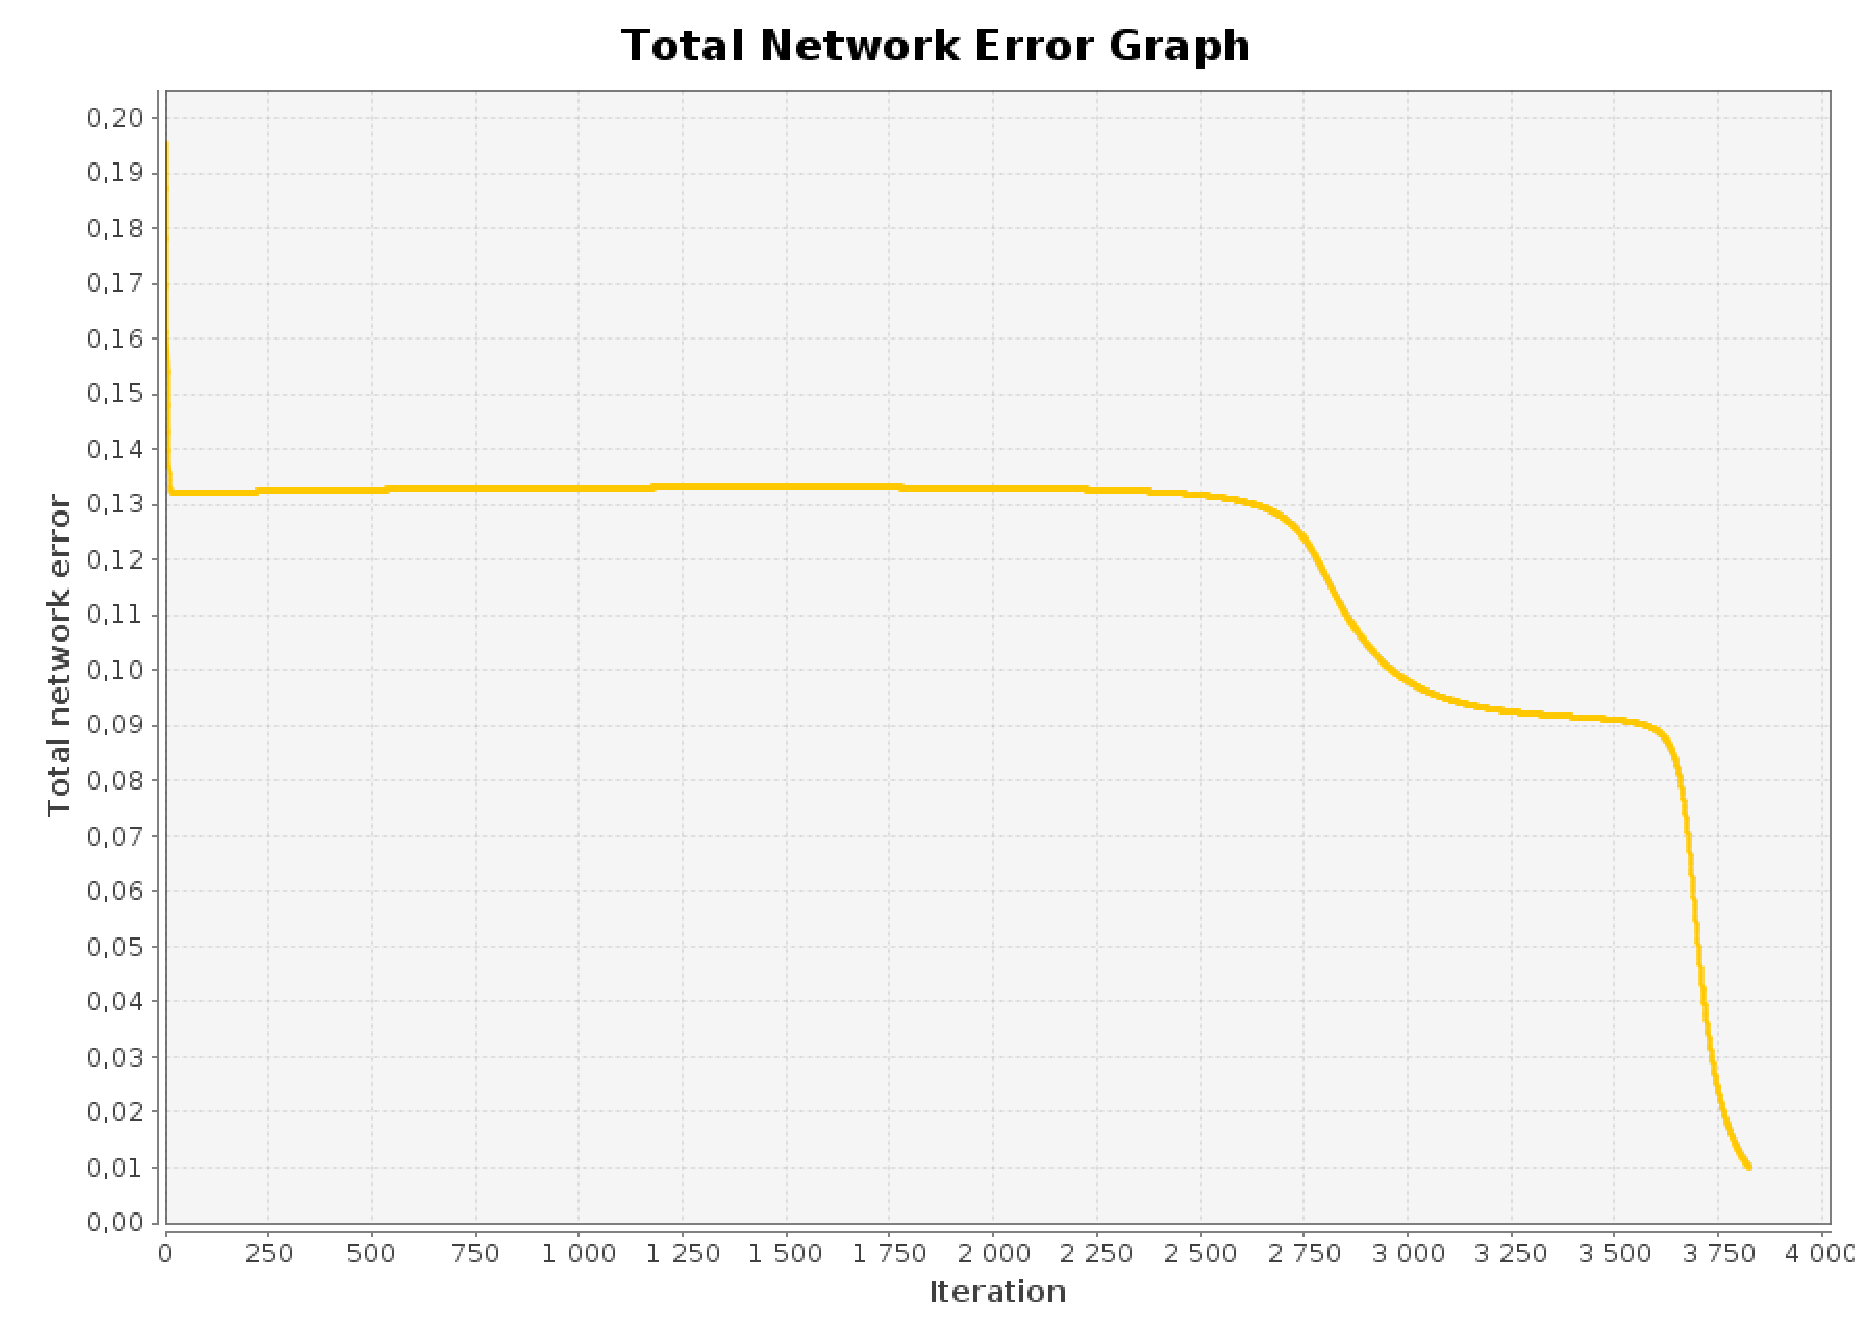
\includegraphics[width=12cm,height=9cm]{./pics/eq/multi_3_3_def.eps}
\caption{Apprentissage fonction "et" avec un pas de 1}
\label{fig:anderr4}
\end{figure}


Rajouter une couche cachée supplémentaire ne semble pas améliorer le nombre d'itération
nécessaire par rapport à un perceptron à une seule couche cachée.

\begin{figure}[h]
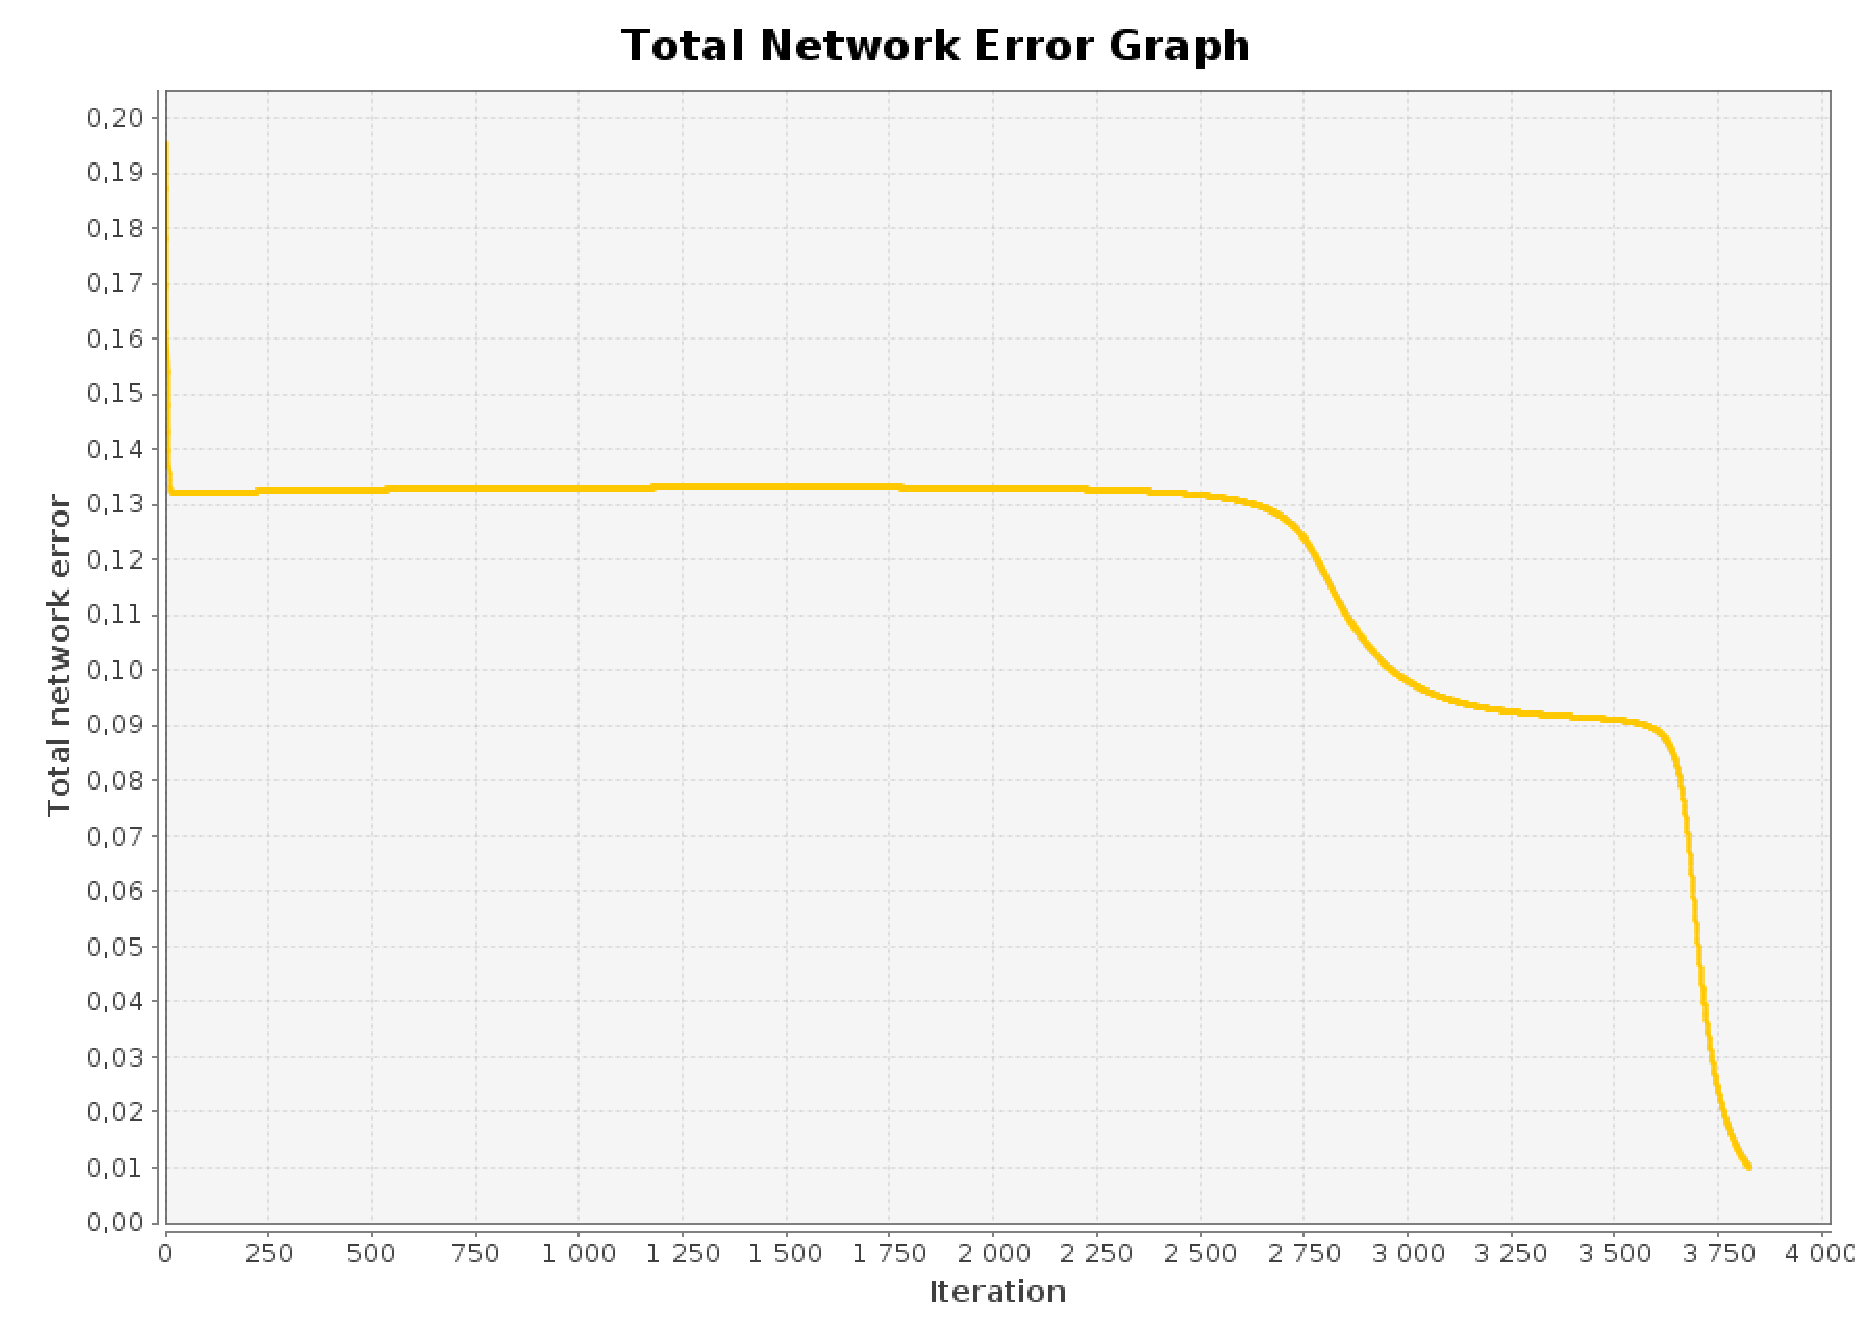
\includegraphics[width=6cm,height=3cm]{./pics/eq/multi_3_3_def.eps}
\caption{Apprentissage fonction "et" avec un pas de 1}
\label{fig:anderr4}
\end{figure}

\begin{figure}[h]
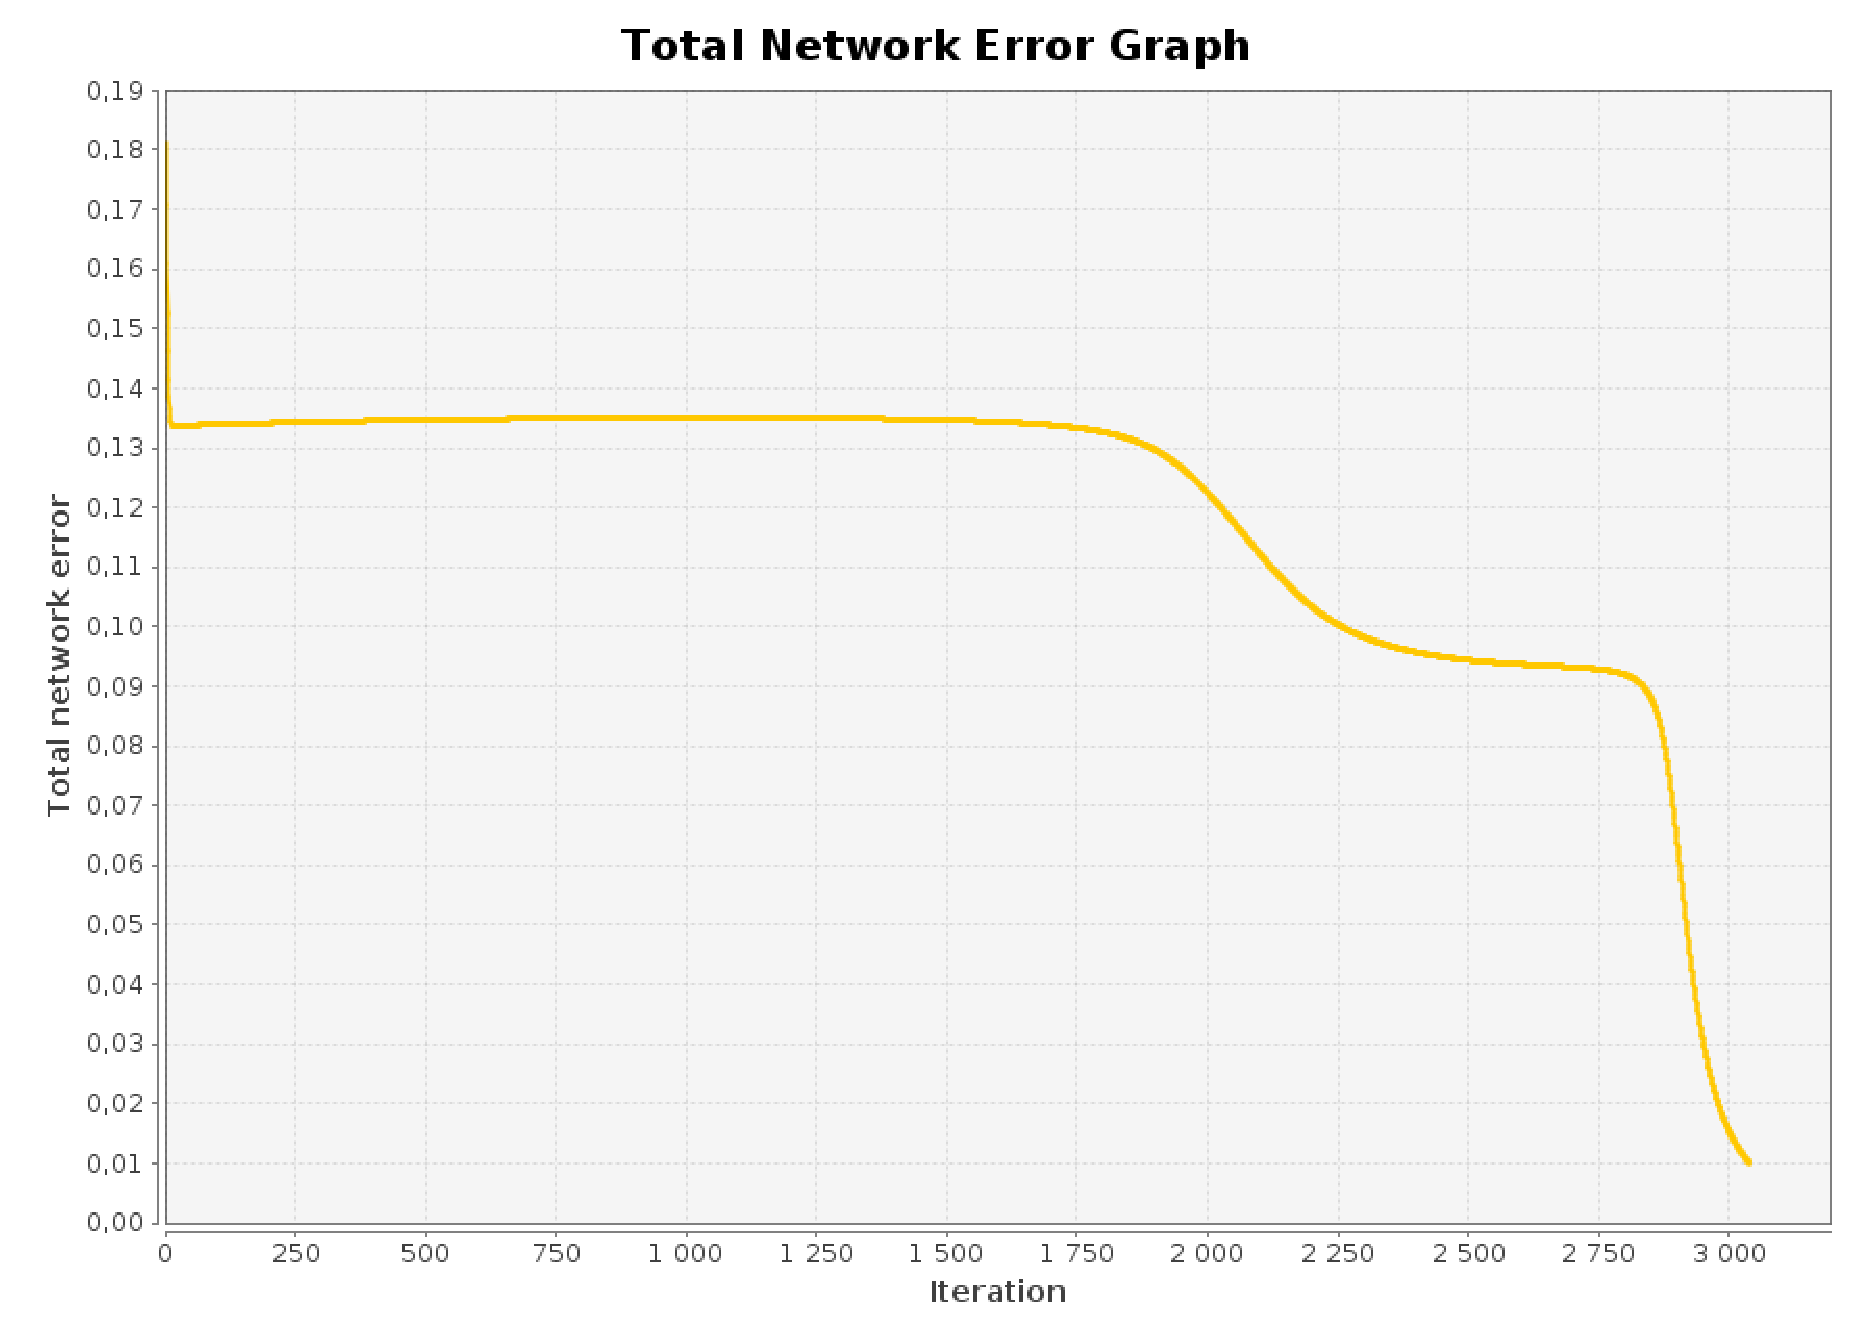
\includegraphics[width=6cm,height=3cm]{./pics/eq/multi_4_4_def.eps}
\caption{Apprentissage fonction "et" avec un pas de 1}
\label{fig:anderr4}
\end{figure}

\begin{figure}[h]
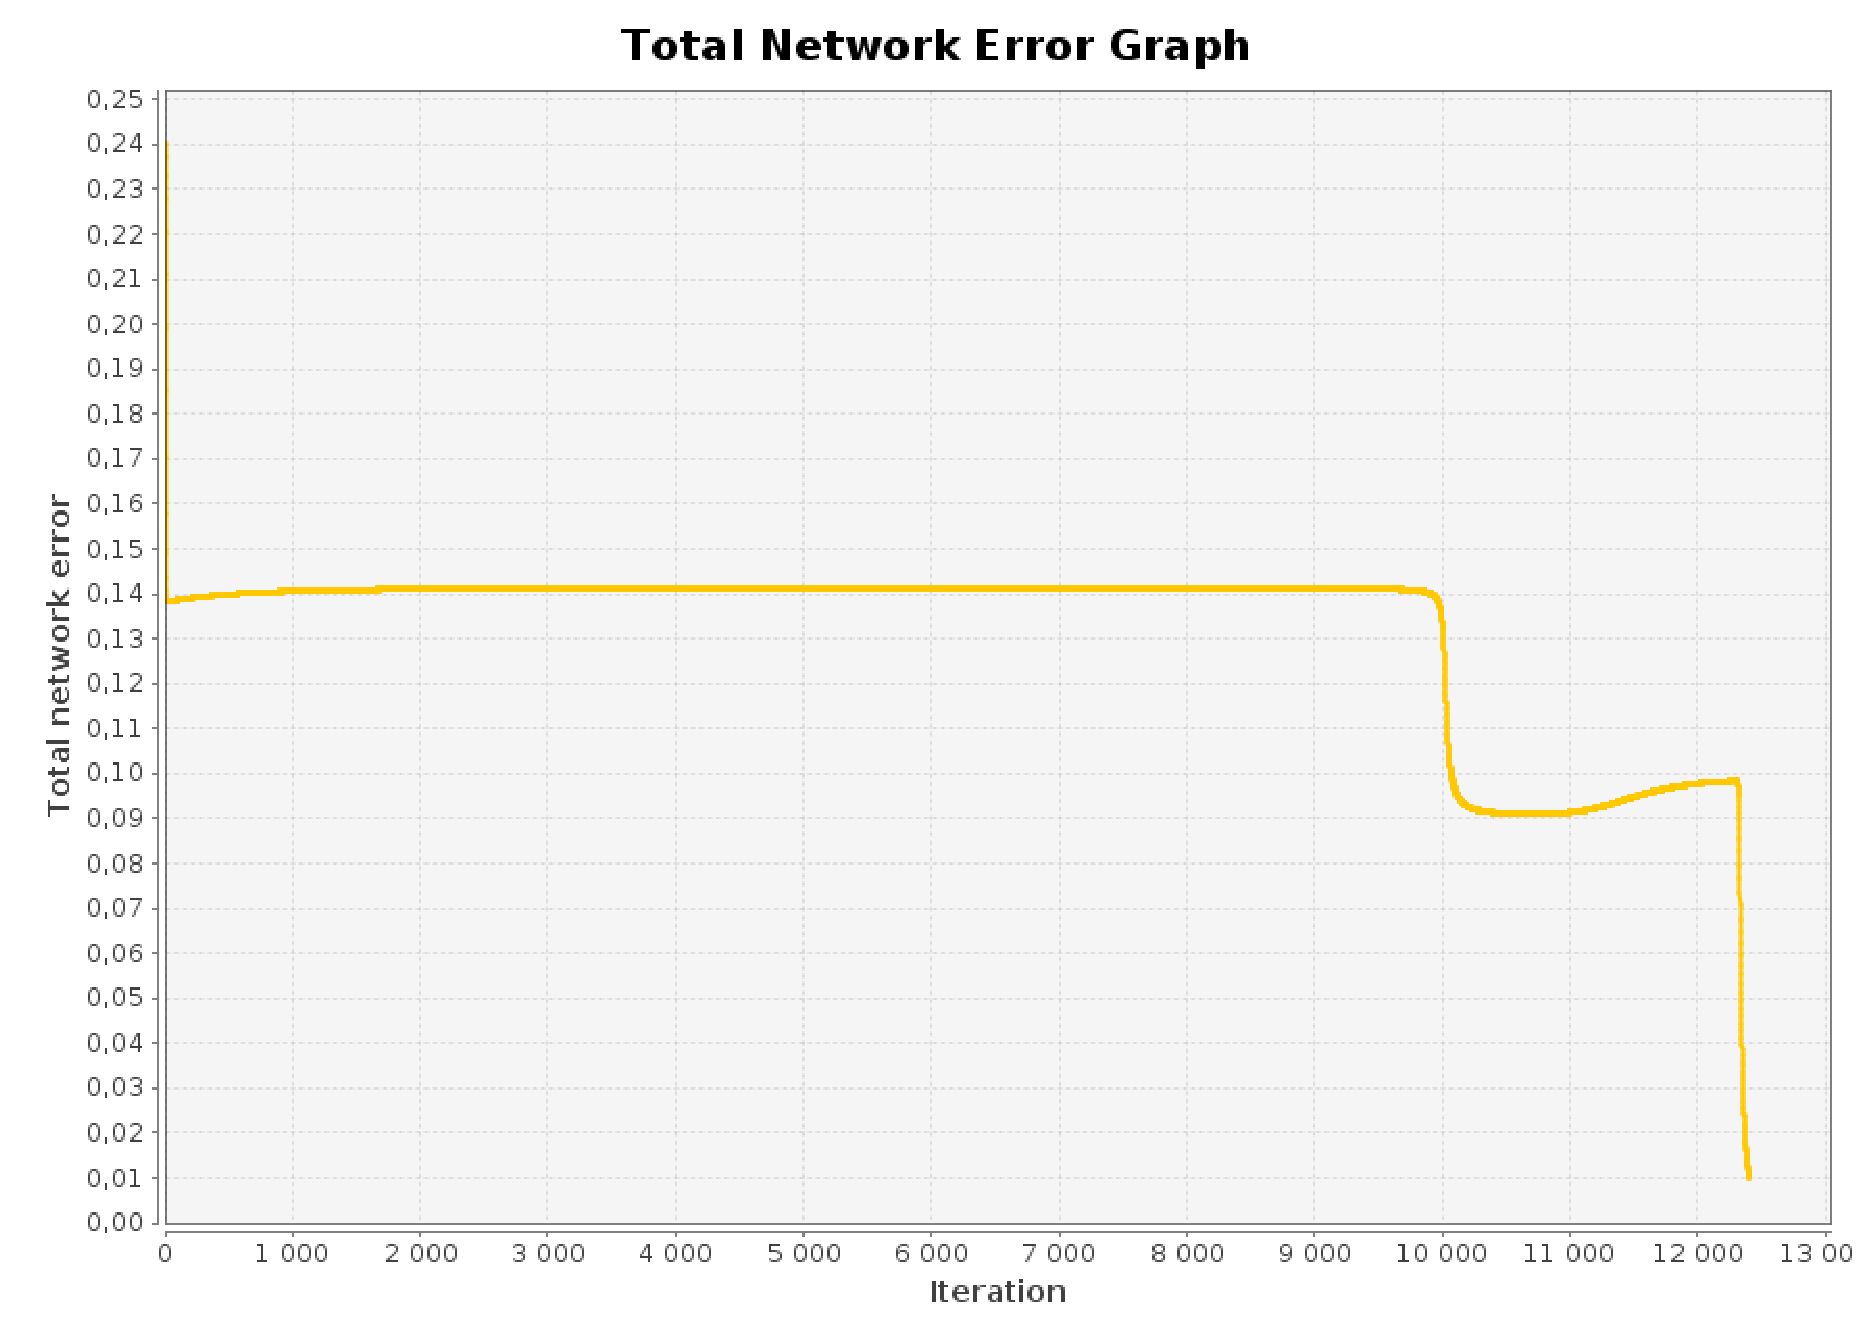
\includegraphics[width=6cm,height=3cm]{./pics/eq/multi_6_6_def.eps}
\caption{Apprentissage fonction "et" avec un pas de 1}
\label{fig:anderr4}
\end{figure}

\begin{figure}[h]
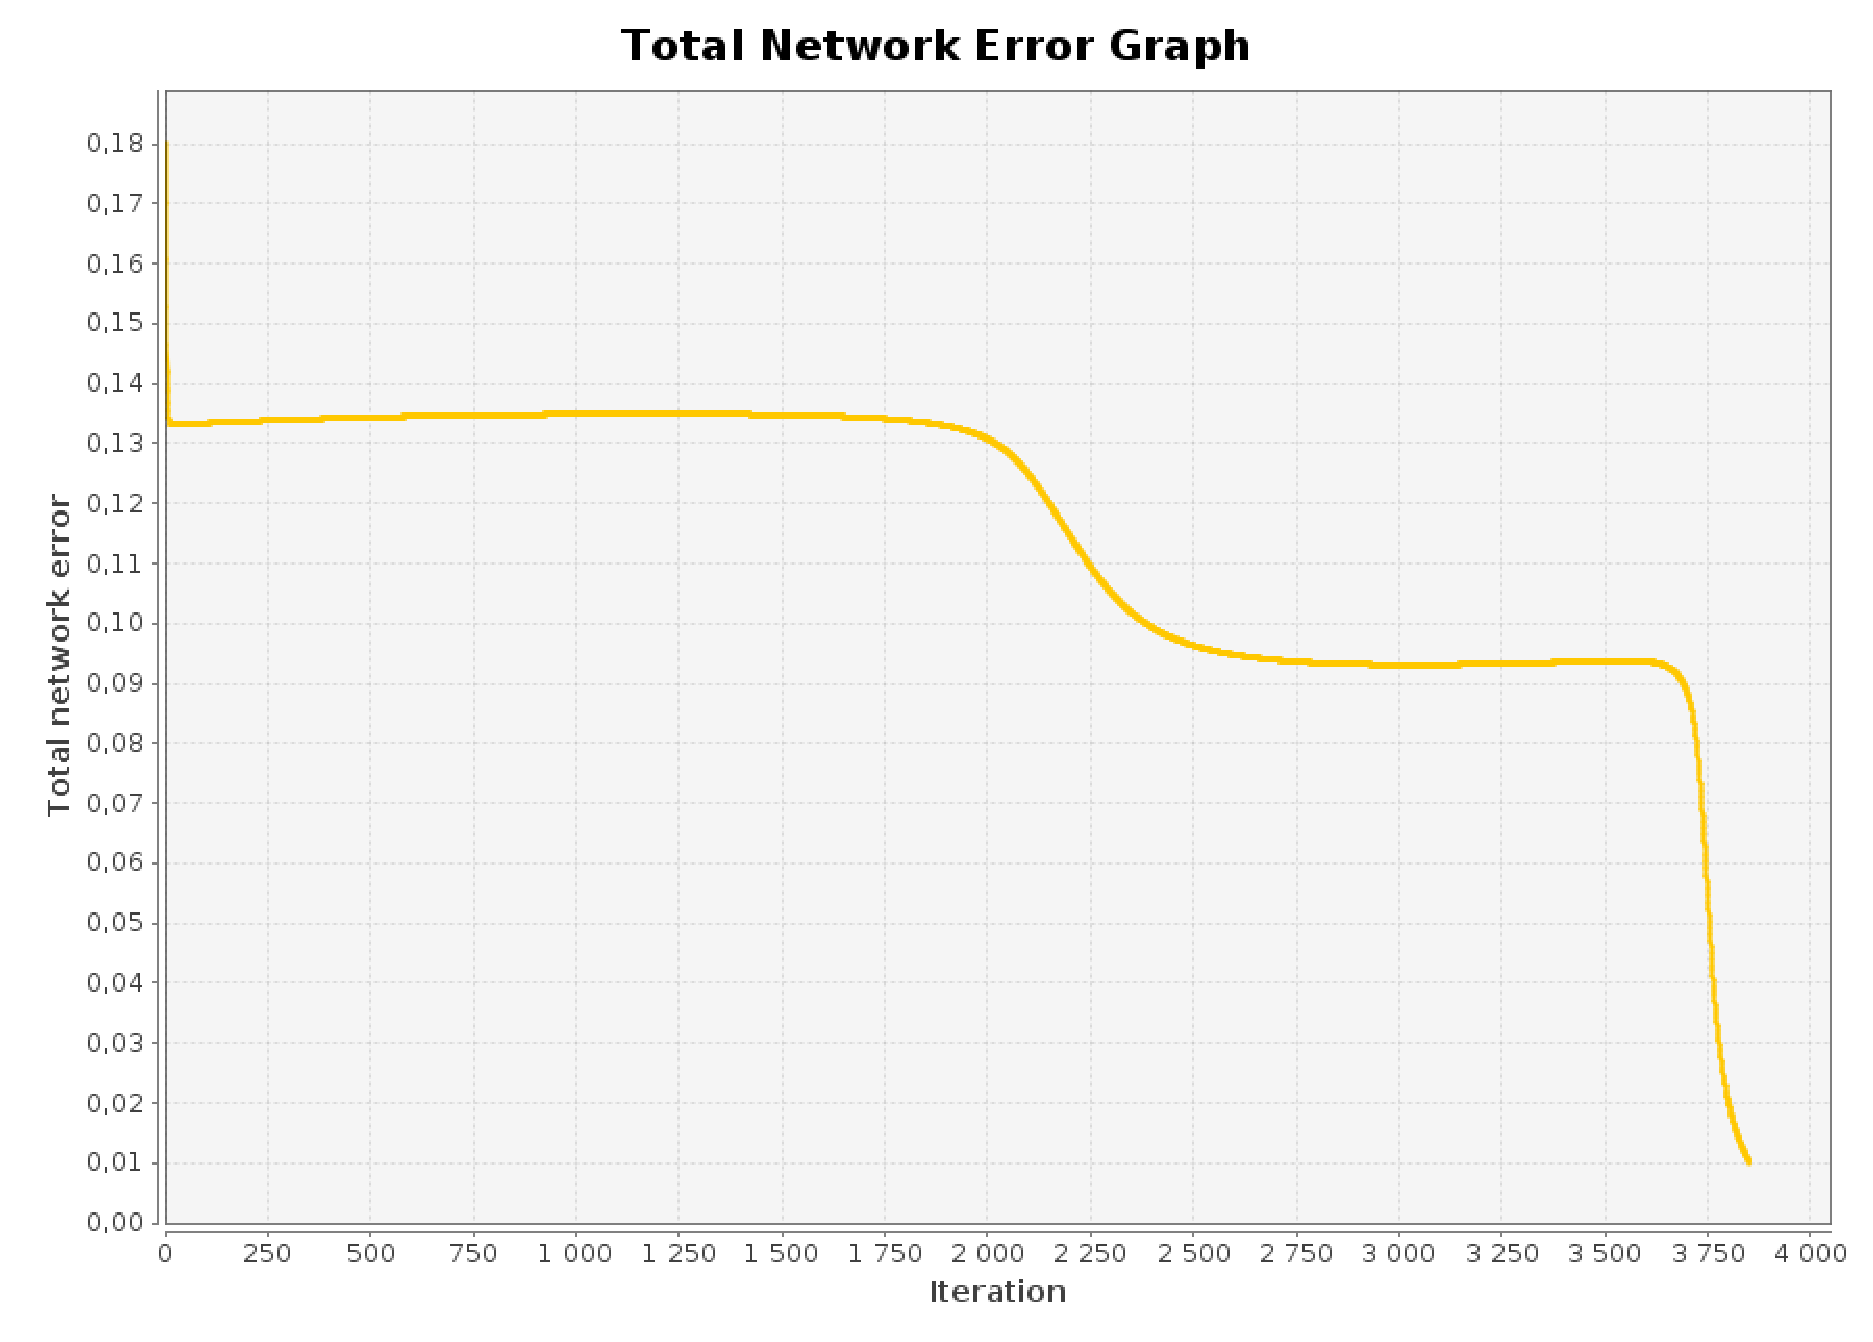
\includegraphics[width=6cm,height=3cm]{./pics/eq/multi_3_4_def.eps}
\caption{Apprentissage fonction "et" avec un pas de 1}
\label{fig:anderr4}
\end{figure}


Rajouter des neurones dans les couche intermédiaire n'améliore pas le résultat non plus.

\begin{figure}[h]
\centering
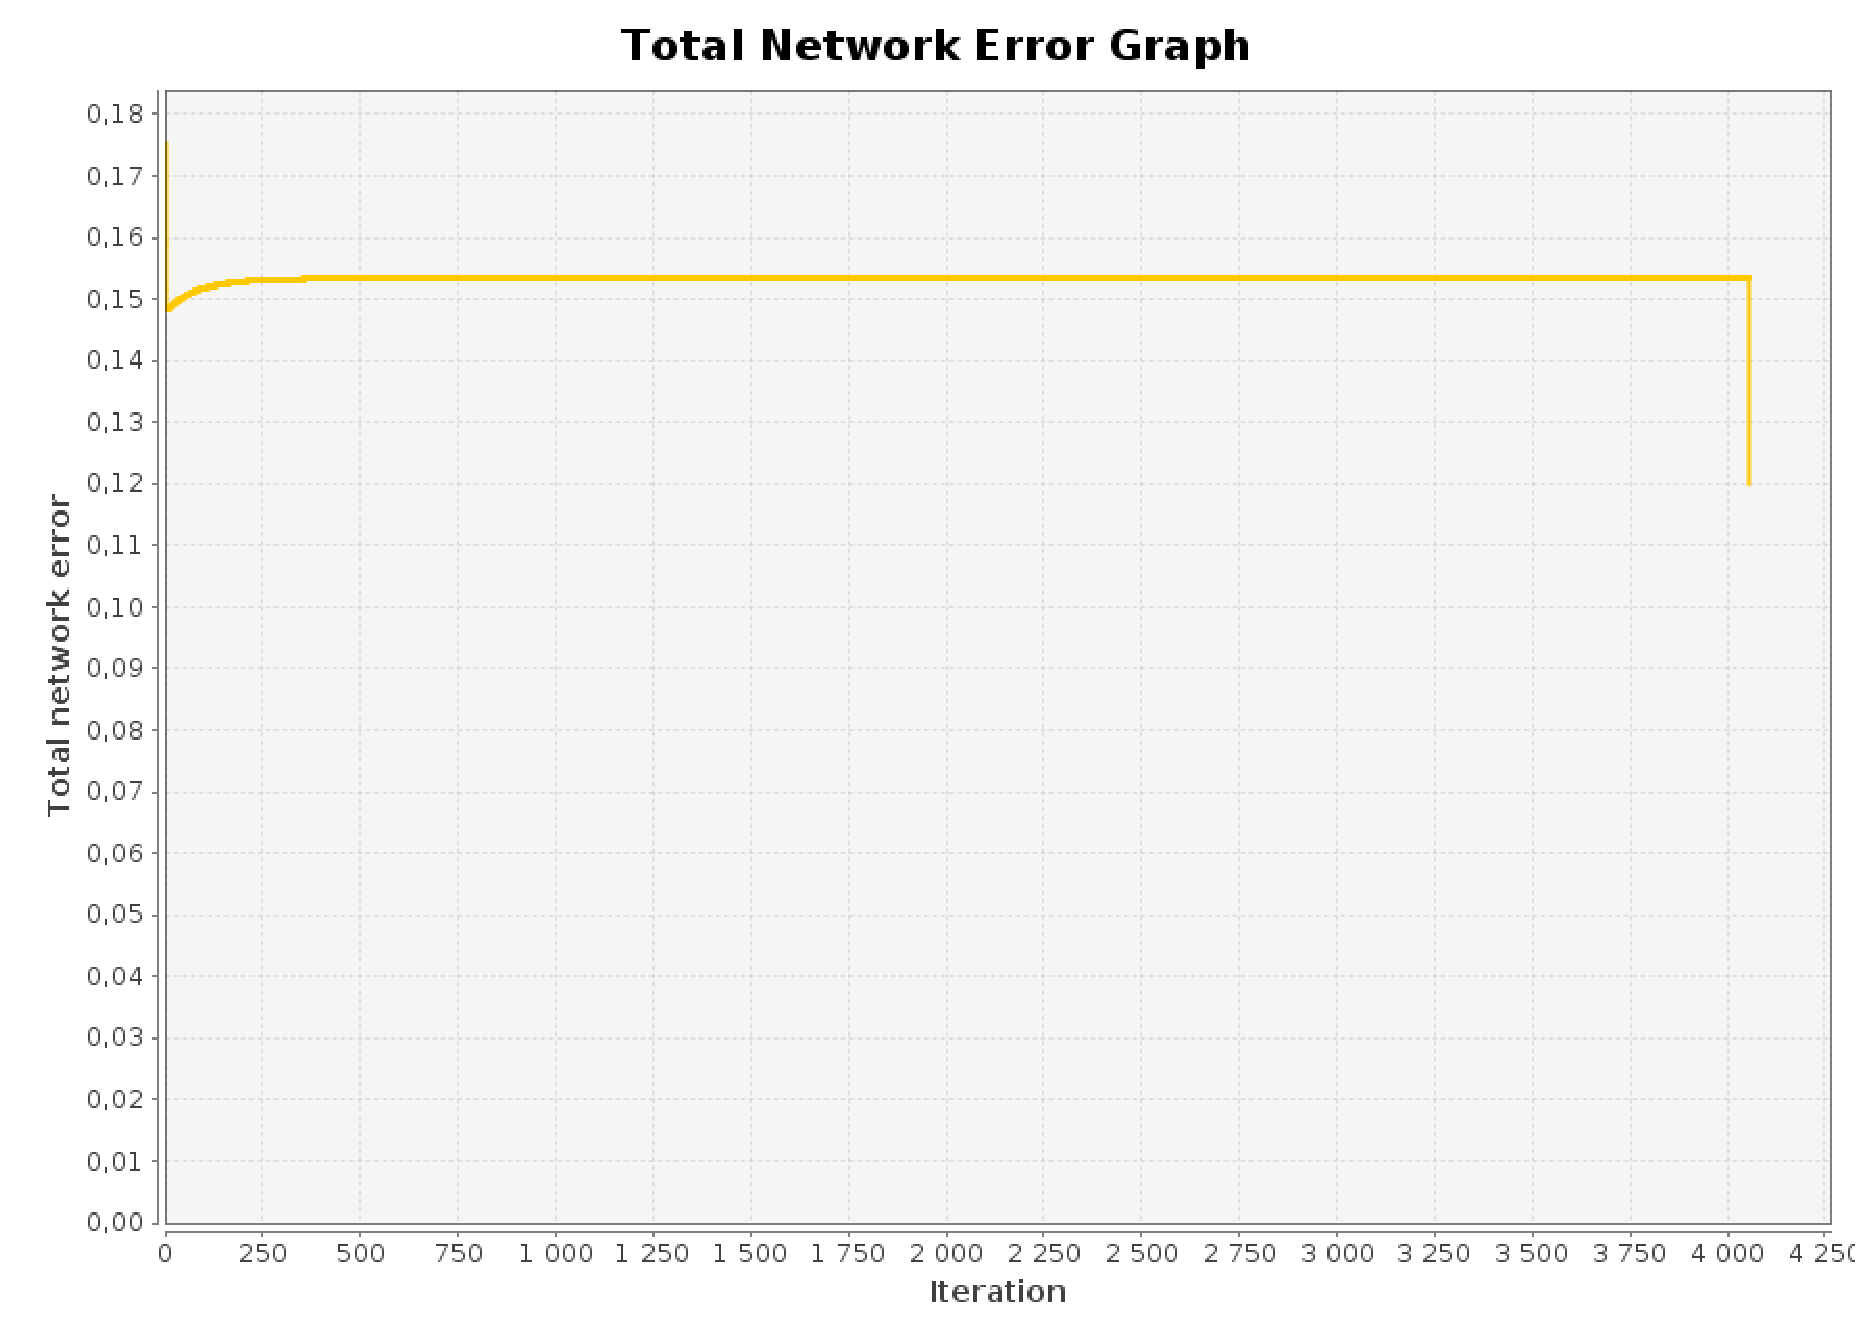
\includegraphics[width=6cm,height=3cm]{./pics/eq/multi_3_3_3_def.eps}
\caption{Apprentissage fonction "et" avec un pas de 1}
\label{fig:anderr4}
\end{figure}


Et rajouter encore une couche fait croitre la courbe jusqu'a ce qu'elle se
stabilise et ne semble plus diminuer.


\section{Apprentissage de la fonction: $f(x) = x^2$}

Il est temps de tester si un perceptron (mono-couche ou multi-couches) est
capable d'apprendre une fonction un peu plus complexe que celle qu'on a vu jusqu'à présent: 
la fonction carré: $f(x) = x^2$ !\\

Plusieurs différences sont à notées par rapport aux fonctions précédentes.
Si avant, le domaine de nos fonctions binaires étaient réduit à ${0,1}$, cette
fois nous sommes confrontés à une fonction continue définie dans tout $\mathbb{R}$.
%TODO if there is time: can we implement a NN in R? %
Une autre différence est liée au type et nombre d'inputs, et change
considérablement le paradigme utilisé par notre réseau:\\

Un concept que nous n'avons pas introduit jusqu'à présent est l'éxistence de plusieur
types de données pour l'apprentissage, et autant de paradigmes d'apprentissage qui en
découlent. Les deux principaux types de données avec lesquels on doit faire
face sont:

\begin{itemize}
\item Des variables catégorielles (dit aussi qualitative) - où il y a généralement
      un ou plusieurs cas qui peuvent être regroupés en différentes catégories 
     (par example: haut, bas ou rouge, vert, bleu, etc.)
\item Des données quantitatives qui se présentes comme une mesure numérique d'un attribut
\end{itemize}

On appelle %TODO%Les types d'apprentissage utilisé pour reconnaitre et classifier des données
appartenant à la première famille "classification". D'un autre côté l'apprentissage
supervisé avec des données quantitatives est appellé "régression".\cite{kindsNN}\\

Pour récapituler: la régression consiste à estimer ou à prédire une réponse,
la classification est l'identification de l'appartenance à un groupe.\\

Dans nos exemples précédents ("et" logique et equivalence) on a simplement
traité des classifications binaires. Cette fois on est confronté avec des données
de type quantitative.


\subsection{Un perceptron pour la fonction $f(x) = x^2$}
Un perceptron n'est pas le moyen plus efficace pour calculer cette 
fonction, mais peut il le faire?\\

Comme nous l'avons vu précédement, un perceptron mono-couche peut être utilisé sans aucun
problème pour distinguer des données linéairement séparables, mais il échoue 
à reconnaitre des schémas un peu plus complexe. Il n'est donc 
probablement adapté à notre problème.\\

Le théorème de l'approximation universelle (aussi connu sous le nom de théoèeme de Cybenko) 
nous dis qu'un perceptron multi-couches avec une seule couche cachée (avec un nombre
fini de neurones) peut approximer n'importe quelle fonction continue dans un 
intervalle de $\mathbb{R}$.
\footnote{
La démonstration mathématique de ce théorème est assez longue et complexe. Une approche visuelle
qui se prête à une demonstration beaucoup plus intuive est proposé à \cite{visuniprof}.
}
\cite{cybthm}

Pour l'apprentissage de la fonction carré nous allons donc utiliser un perceptron
multi-couche avec une seule couche cachée et on cherchera à lui faire apprendre
la fonction carré dans un intervalle de $\mathbb{R}$.

Pour commencer on pourra utiliser un perceptron avec 3 neurones cachés comme
celui que l'on a utilisé précédement pour l'équivalence. Notre but sera
d'approximer la fonction carré dans l'intervalle $[1,100]$.

Dans notre exemple chaque neurone de notre perceptron utilisera la fonction
d'activation sigmoide, c'est pour cette raison que l'on normalisera les inputs
d'apprentissage pour les borner entre l'intervalle $[0,1]$ (codomaine de la
fonction sigmoide).

\subsubsection{3 neurons cache}

Pour ne pas surcharger notre  perceptron on pourrait commencer à tester
ses capacités d'apprentissage avec un dataset de dimensions réduites (table
\ref{tab:fqt1}). On rappelle que pour avoir un data set compris entre 0 et 1
nous avons normalisé notre data set.

\begin{table}[h]
  \centering
  \begin{tabular}{| c | c |}
    \hline
    \textbf{$x$} & \textbf{$f(x)$}\\
    \hline
    0 & 0 \\
    \hline
    10 & 100 \\
    \hline
    20 & 400 \\
    \hline
    ... & ... \\
    \hline
    100 & 10000 \\
    \hline
  \end{tabular}
  \caption{Fontion carre: dataset 1}
  \label{tab:fqt1}
\end{table}

Avec les valeurs par défaut pour l'apprentissage, notre réseau arrive à obtenir
un bon taux d'erreur dans un temps raisonable comme le montre la figure
\ref{fig:sqtest1}. Après ce premier test notre réseau nous offre déjà une
approximation appréciable de la fonction carré (figure \ref{fig:chartsqtest1}).

\begin{figure}[h]
\centering
\includegraphics[width=12cm,height=9cm]{./pics/sqtest1.eps}
\caption{Apprentissage fonction carré: 3 neurons, dataset 1}
\label{fig:sqtest1}
\end{figure}

\begin{figure}[h]
\centering
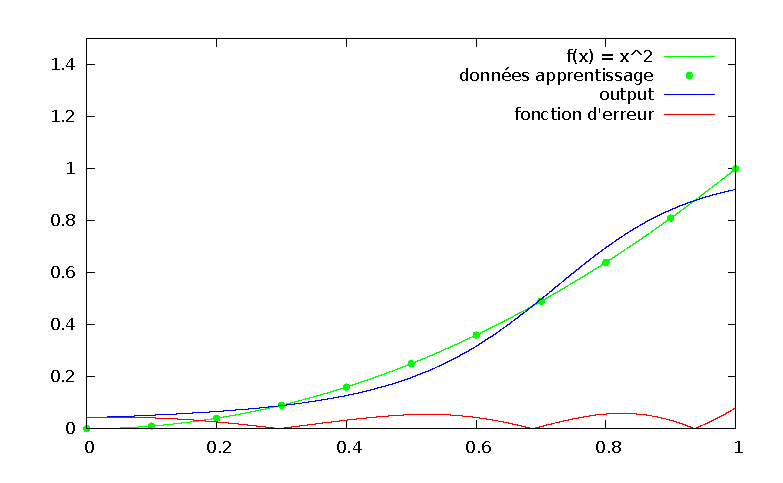
\includegraphics[width=12cm,height=9cm]{./pics/chartsqtest1.eps}
\caption{Résultat apprentissage: 3 neurons, dataset 1}
\label{fig:chartsqtest1}
\end{figure}

Maintenant nous pouvons essayer d'augmenter la précision de notre dataset
pour essayer d'obtenir une meilleure approximation. Pour notre 
prochain test on essayera de doubler la précision de notre dataset.
Les figures \ref{fig:sqtest2} et \ref{fig:chartsqtest2} nous montre 
une amélioration sensible des performances de notre réseau. 



\begin{figure}[h]
\centering
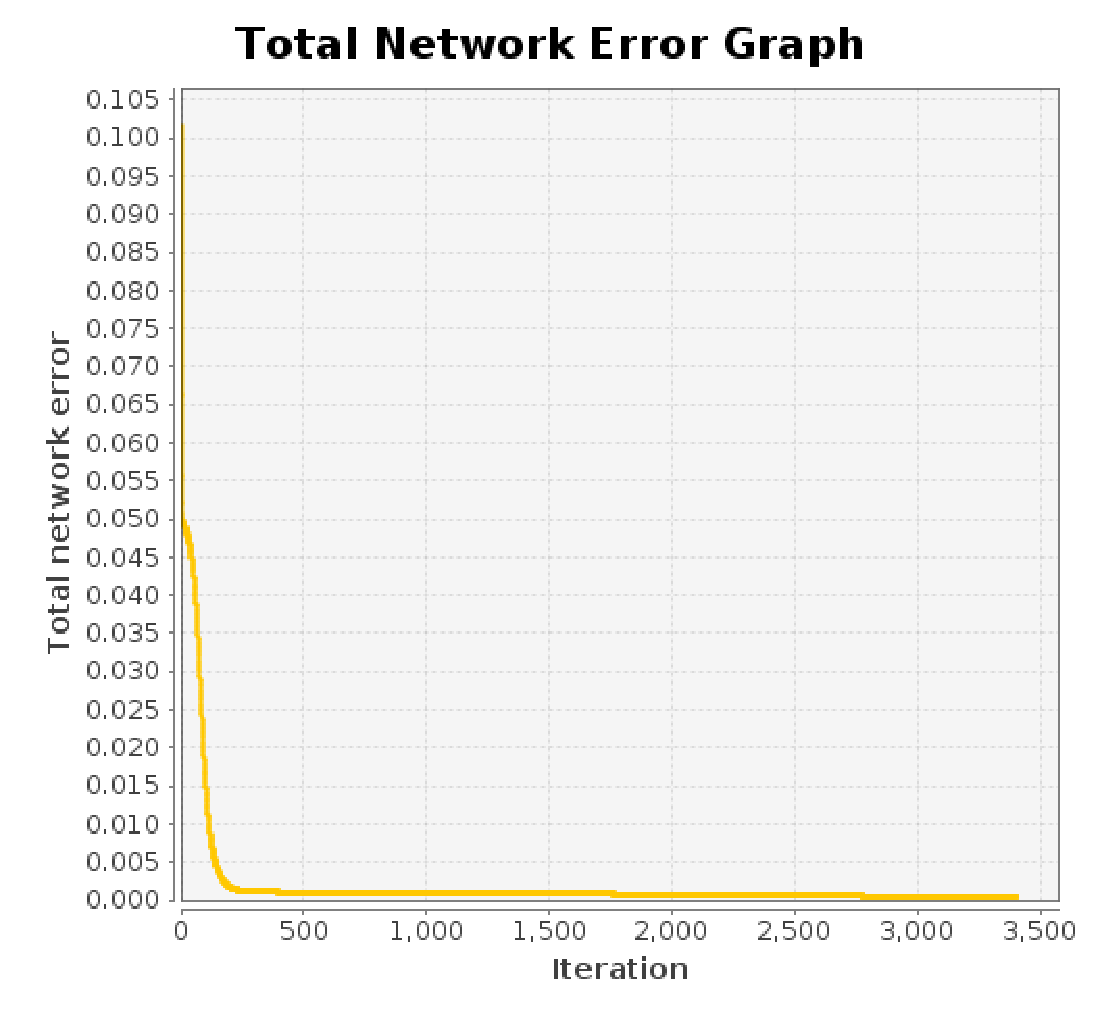
\includegraphics[width=12cm,height=9cm]{./pics/sqtest2.eps}
\caption{Apprentissage fonction carré: 3 neurons, dataset 2}
\label{fig:sqtest2}
\end{figure}

\begin{figure}[h]
\centering
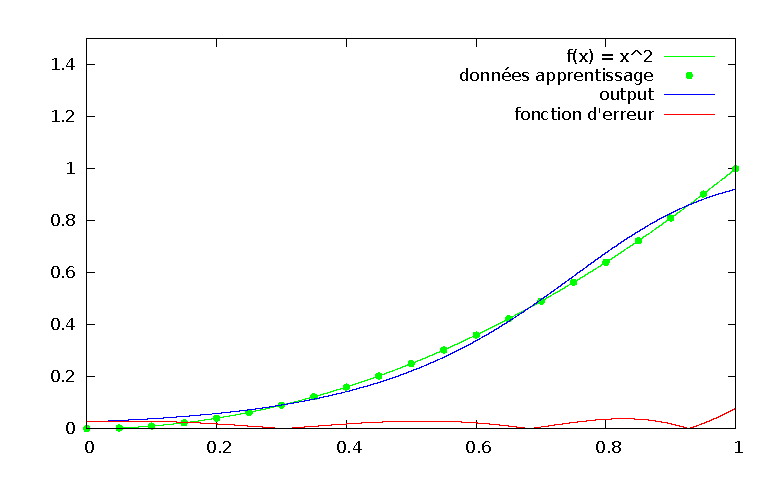
\includegraphics[width=12cm,height=9cm]{./pics/chartsqtest2.eps}
\caption{Resultat apprentissage: 3 neurons, dataset 2}
\label{fig:chartsqtest2}
\end{figure}

Par contre on se rend très vite compte que notre réseau commence à être aux limites
de ces capacités.
Après un certain temps, la vitesse d'apprentissage ralentit beaucoup, 
ce qui implique plusieurs milliés d'itérations pour améliorer de façon 
significative notre approximations (la figure \ref{fig:chartsqtest3} nous
montre les résultats en poursuivant l'entrainement de notre réseau jusqu'à
environ 30.000 époques).La fonction d'erreur est déjà assez proche de son minimum 
globale, c'est donc le moment de passer à un réseau un peu plus grand
et donc avec plus de capacites de stockage.


\begin{figure}[h]
\centering
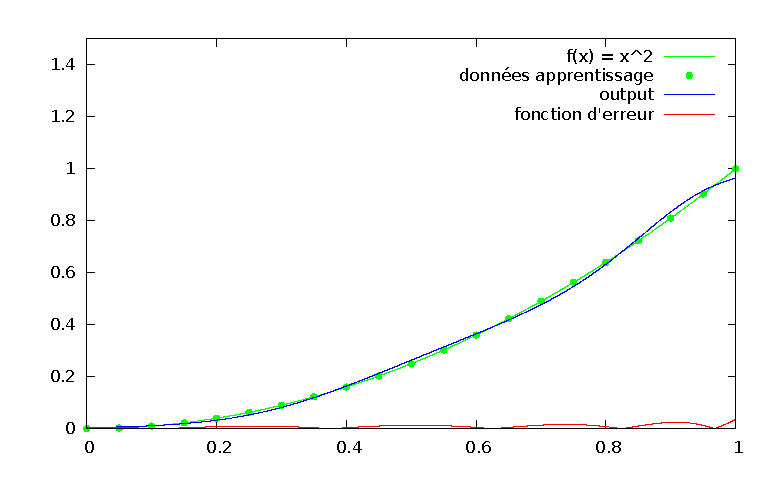
\includegraphics[width=12cm,height=9cm]{./pics/chartsqtest3.eps}
\caption{Résultat apprentissage: 3 neurones, dataset 2, 30.000 iterations}
\label{fig:chartsqtest3}
\end{figure}


\subsubsection{4 neurones cachés}

Avec un réseau de 4 neurones cachés, plus ou moin 10.000 itérations
sont suffisantes pour obtenir un resultat qui dépasse celui obtenu
précedement avec une couche de 3 neuronés et 30.000 itérations 
(figures \ref{fig:sqtest4} et \ref{fig:chartsqtest4}).


\begin{figure}[h]
\centering
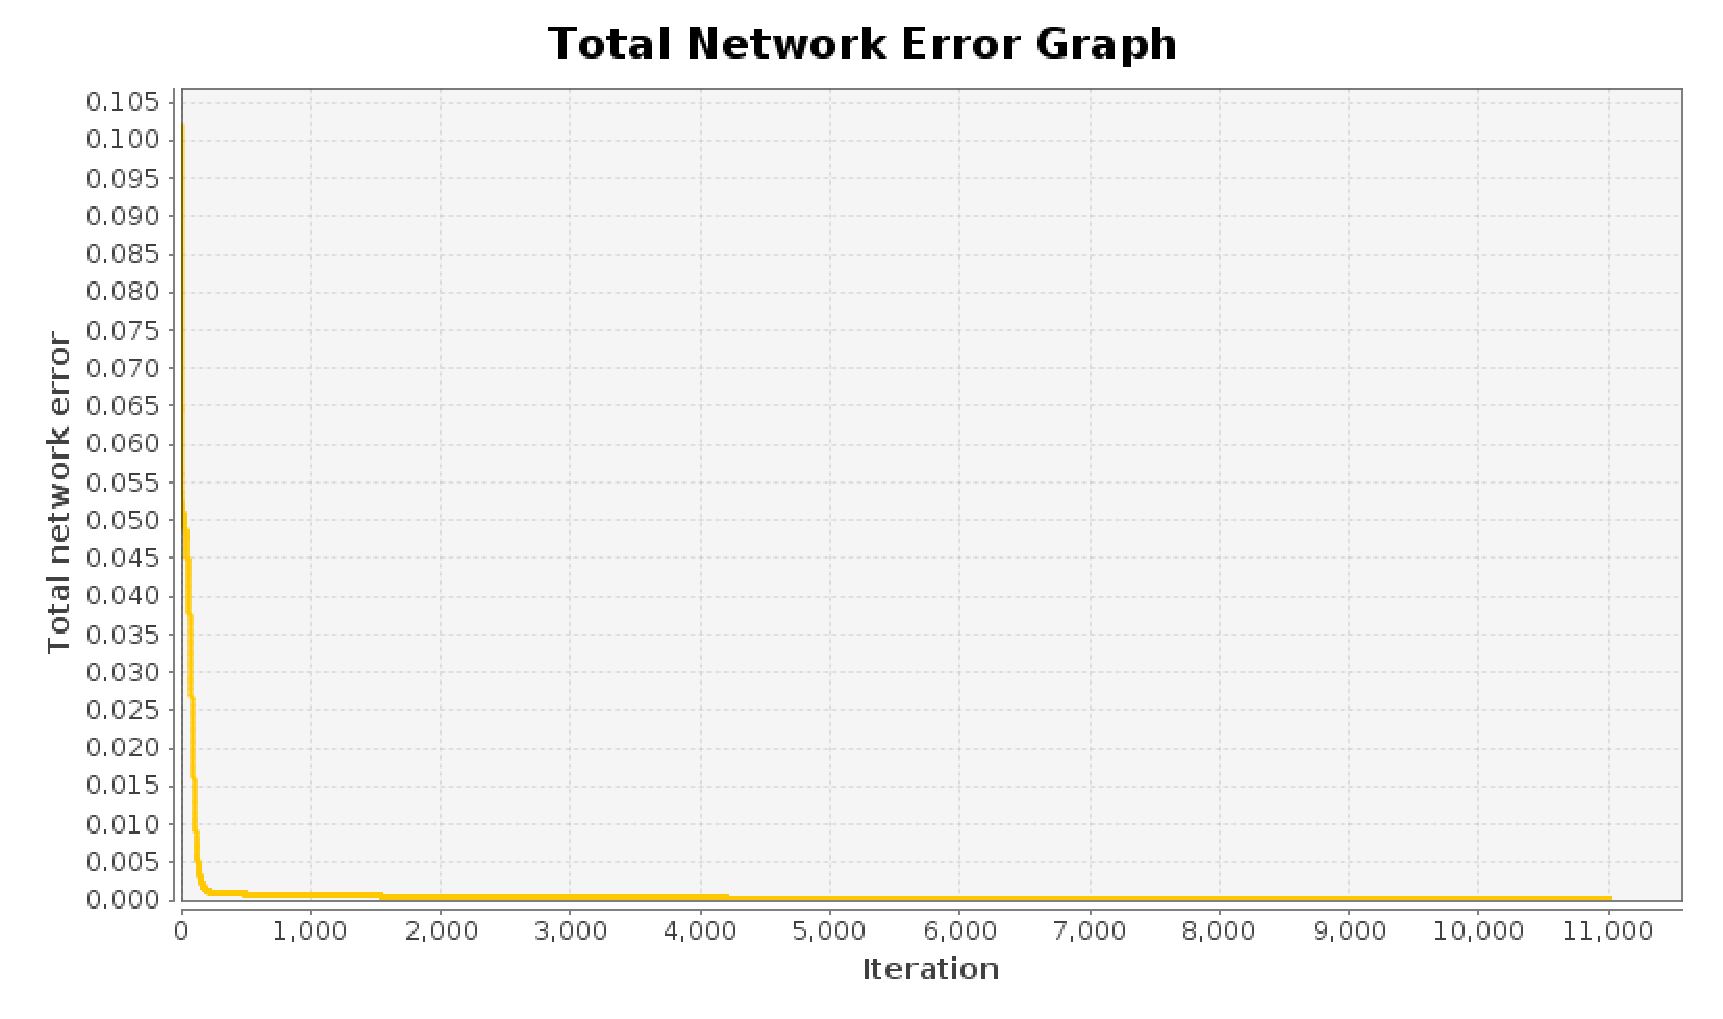
\includegraphics[width=12cm,height=9cm]{./pics/sqtest4.eps}
\caption{Apprentissage fonction carré: 4 neurones, dataset 2}
\label{fig:sqtest4}
\end{figure}

\begin{figure}[h]
\centering
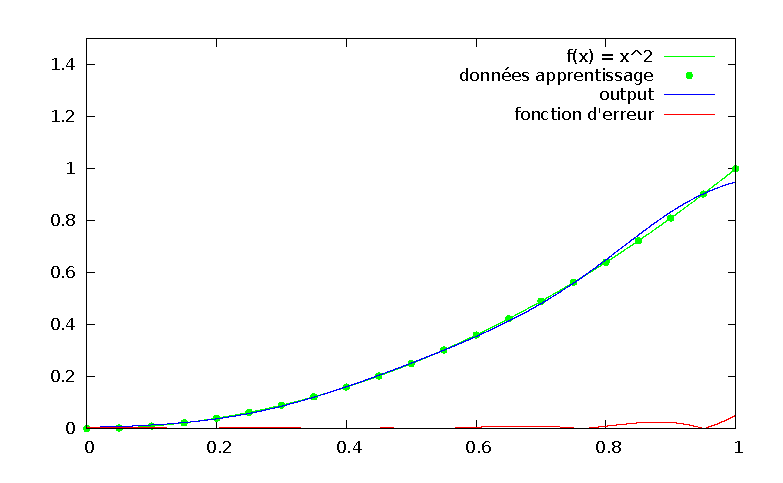
\includegraphics[width=12cm,height=9cm]{./pics/chartsqtest4.eps}
\caption{Résultat apprentissage: 4 neurones, dataset 2}
\label{fig:chartsqtest4}
\end{figure}

Avec un dataset encore plus grand (100 inputs) et après environ
30.000 itérations, on arrive à obtenir une approximation suffisament
précise (fig \ref{chartsqtest5}) comme supposé par le théorème de Cybenko:
un perceptron multicouche avec une seule couche cachée est suffisant pour
approximer la fonction carré (comme n'importe quelle fonction continue) 
et la précision dépend strictement du nombre de neurones dans la couche caché.

\begin{figure}[h]
\centering
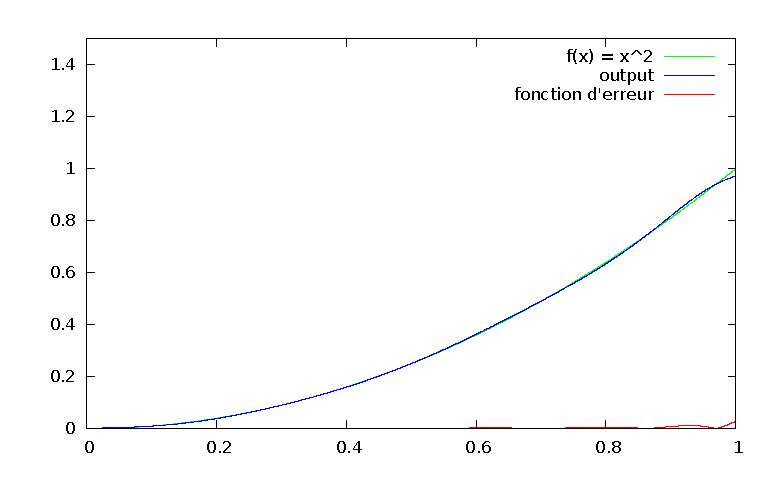
\includegraphics[width=12cm,height=9cm]{./pics/chartsqtest5.eps}
\caption{Resultats apprentissage: 4 neurons, dataset 2}
\label{fig:chartsqtest5}
\end{figure}


%End content
\clearpage
\addcontentsline{toc}{section}{Références}
\bibliographystyle{plain}
\bibliography{rapport}

\end{document}
